
%%%----------------------------------------------------------
%%%----------------------------------------------------------
%%%----------------------------------------------------------
%%%----------------------------------------------------------
%%%----------------------------------------------------------
\chapter{Elevator}
%%%----------------------------------------------------------

The activity "elevator" will be analyzed here with graphics.
%%%----------------------------------------------------------
\section{Test case 1}
%%%----------------------------------------------------------
Test case 1 in Fig.~\ref{fig:Test_case_elevator_1}
\begin{figure}
	\centering\small
	\setlength{\tabcolsep}{0mm}	% alle Spaltenränder auf 0mm
	\begin{tabular}{c@{\hspace{12mm}}c} % mittlerer Abstand = 12mm
		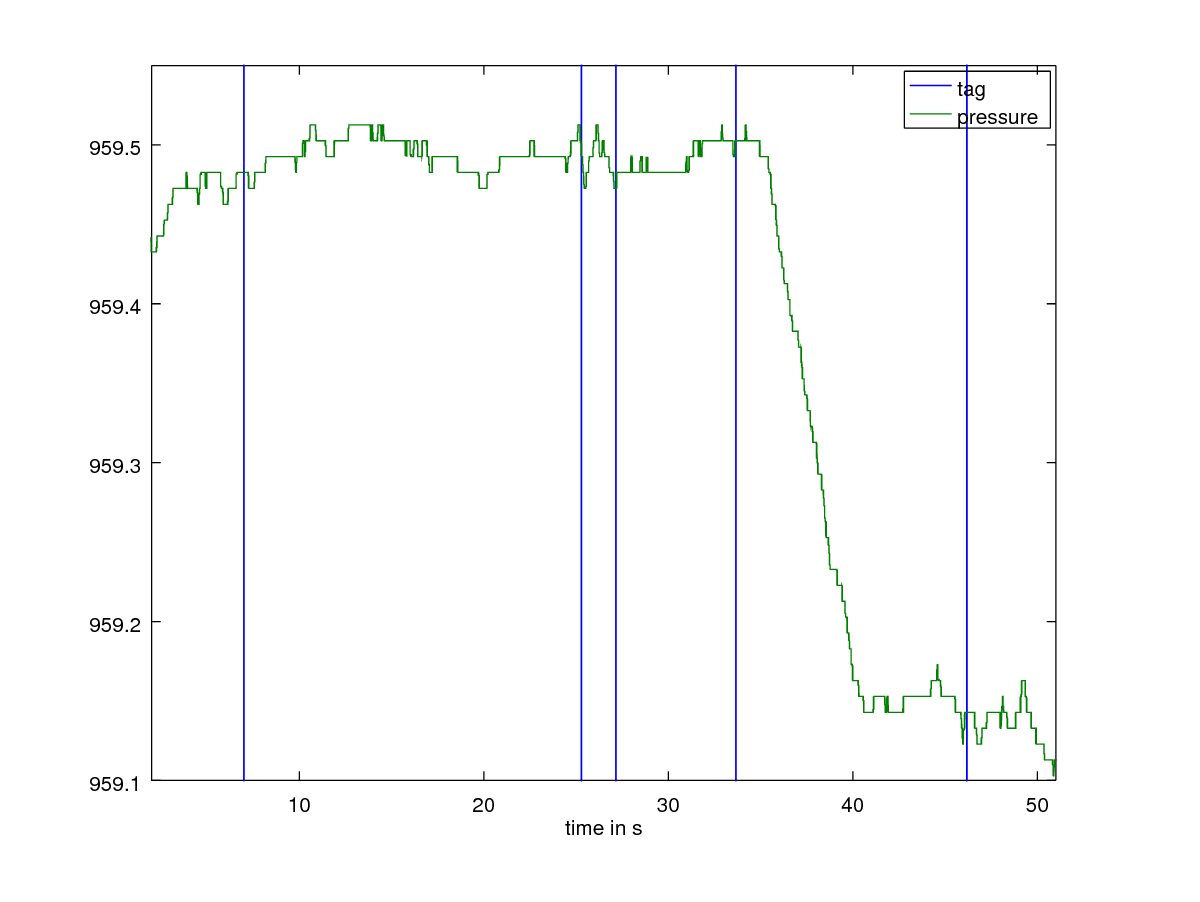
\includegraphics[width=.45\textwidth]{eleuppp99_p} &
		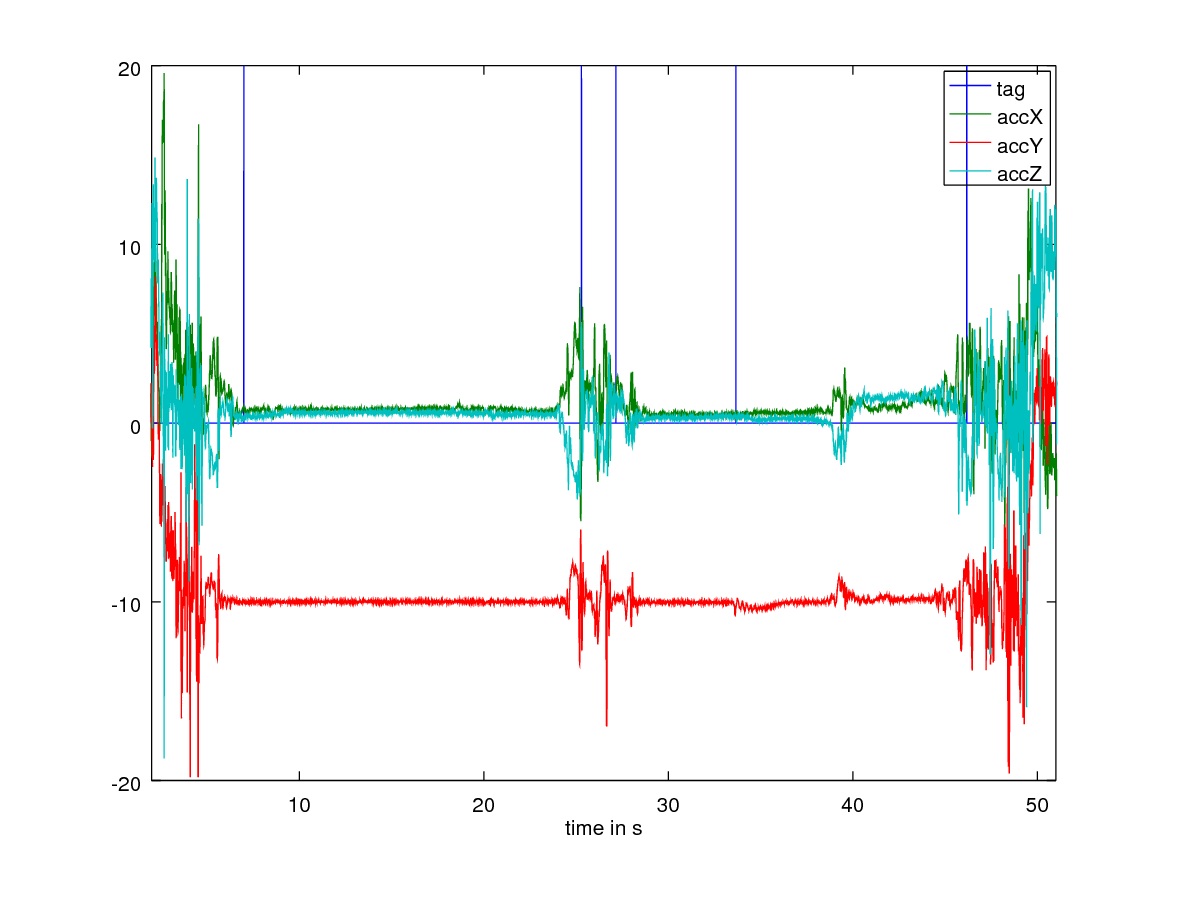
\includegraphics[width=.45\textwidth]{eleuppp99_a} 
		\\
		(a) & (b)
		\\[4pt]	%vertical extra spacing (4 points)
		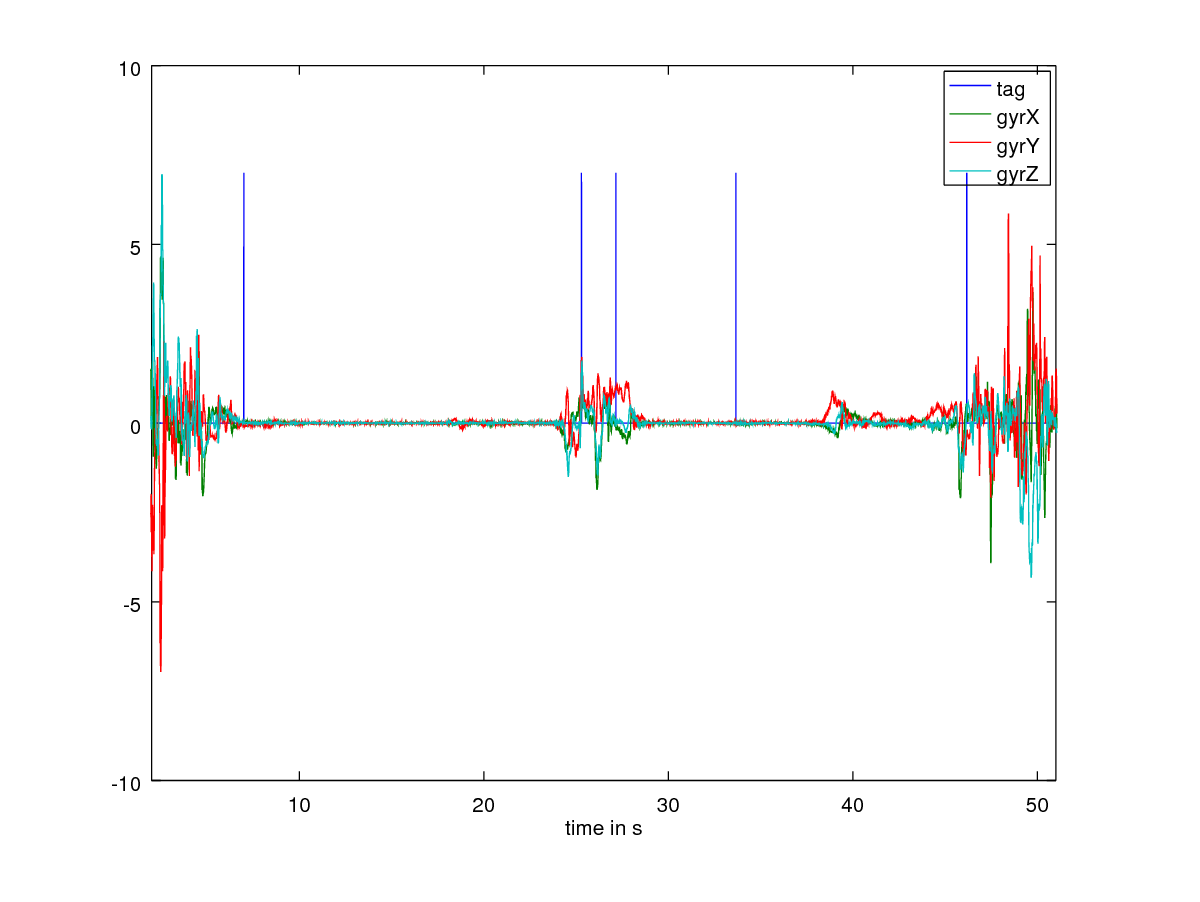
\includegraphics[width=.45\textwidth]{eleuppp99_g} &
		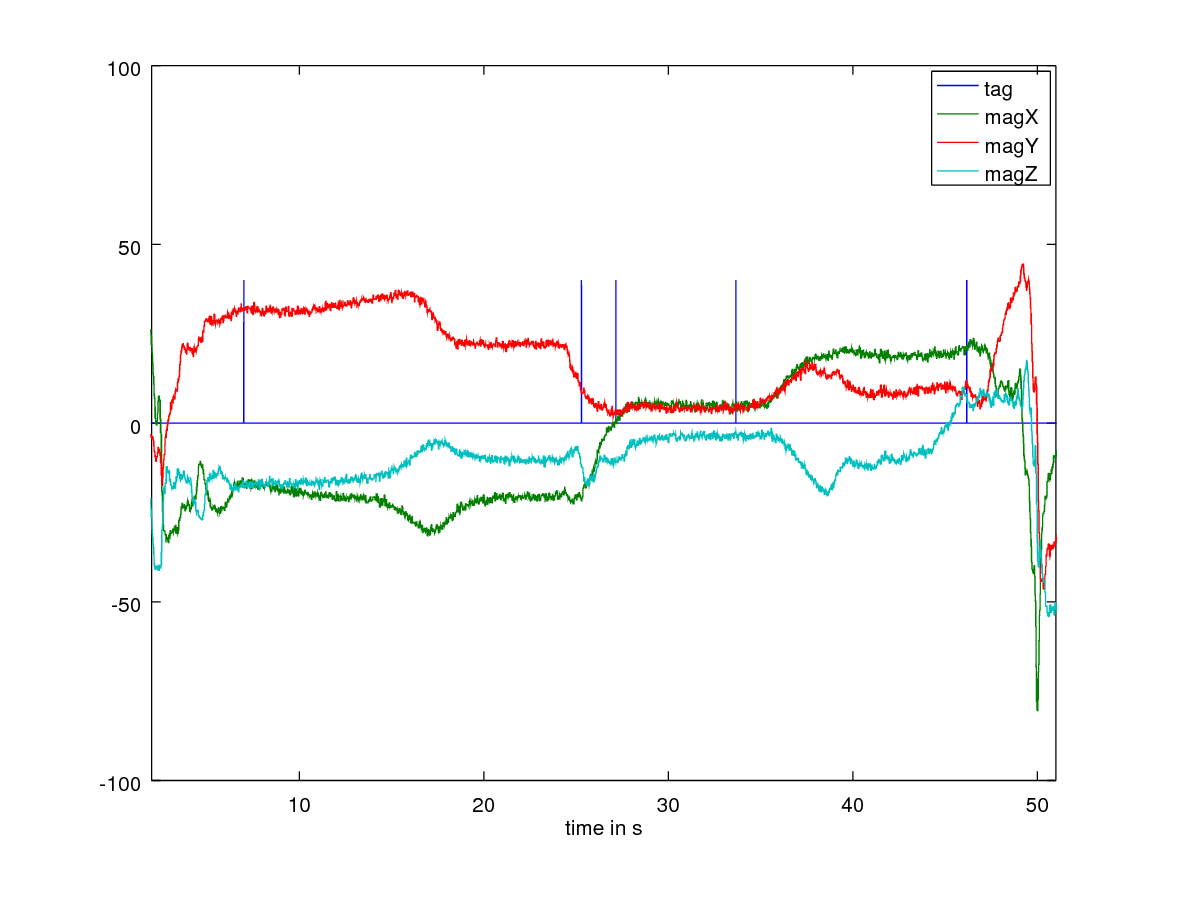
\includegraphics[width=.45\textwidth]{eleuppp99_m} 
		\\
		(c) & (d)

	\end{tabular}
	%
	\caption{Test case 1}
	\label{fig:Test_case_elevator_1}
\end{figure}

%%%----------------------------------------------------------
\section{Test case 2}
%%%----------------------------------------------------------

Test case 2 in Fig.~\ref{fig:Test_case_elevator_2}
\begin{figure}
	\centering\small
	\setlength{\tabcolsep}{0mm}	% alle Spaltenränder auf 0mm
	\begin{tabular}{c@{\hspace{12mm}}c} % mittlerer Abstand = 12mm
		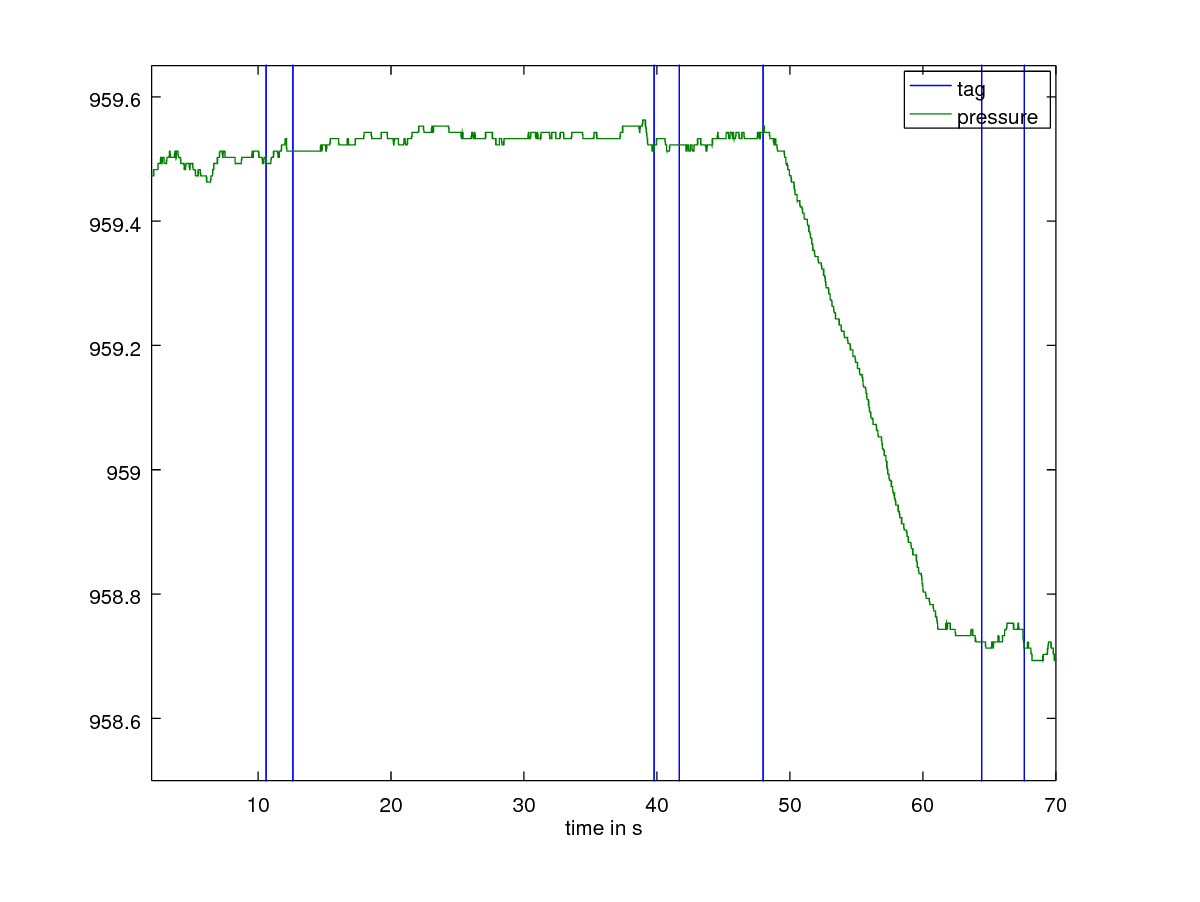
\includegraphics[width=.45\textwidth]{eleup12_p} &
		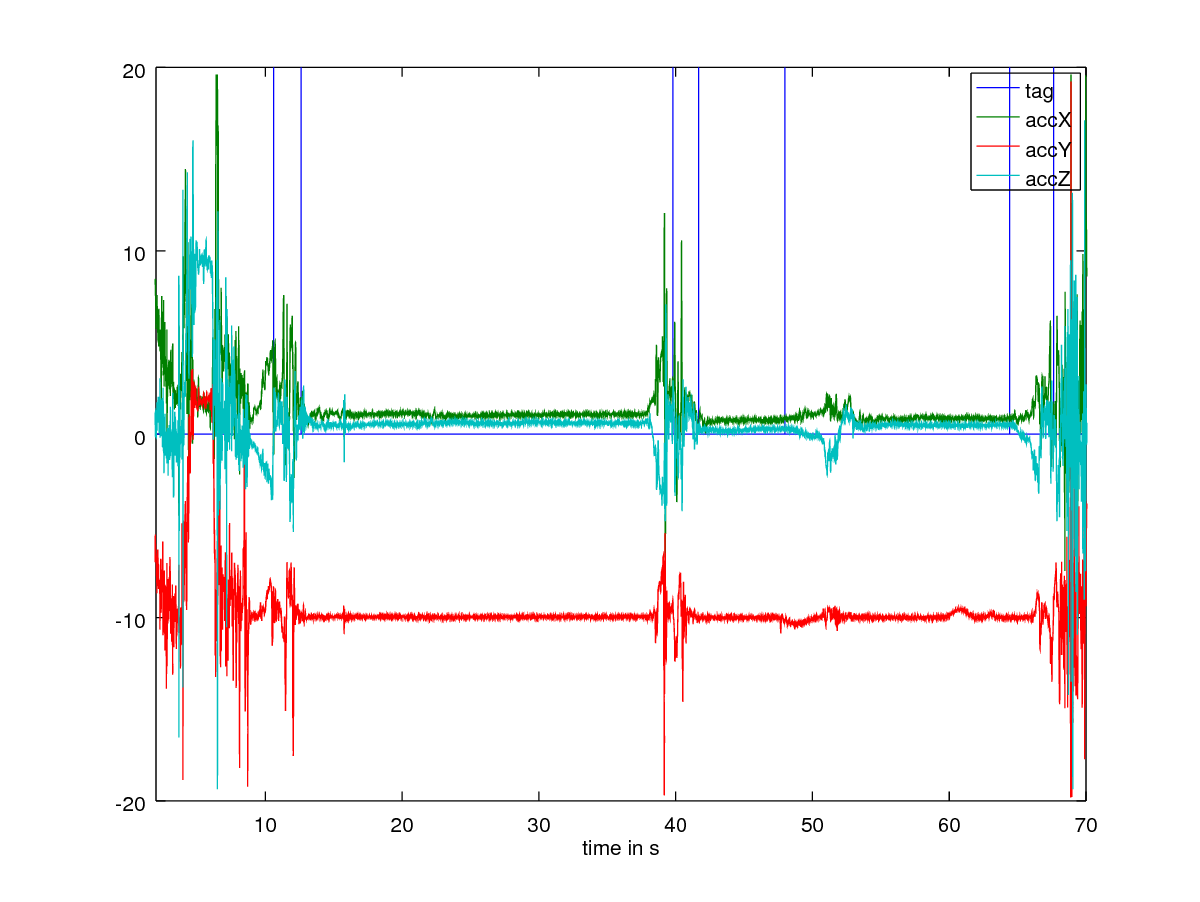
\includegraphics[width=.45\textwidth]{eleup12_a} 
		\\
		(a) & (b)
		\\[4pt]	%vertical extra spacing (4 points)
		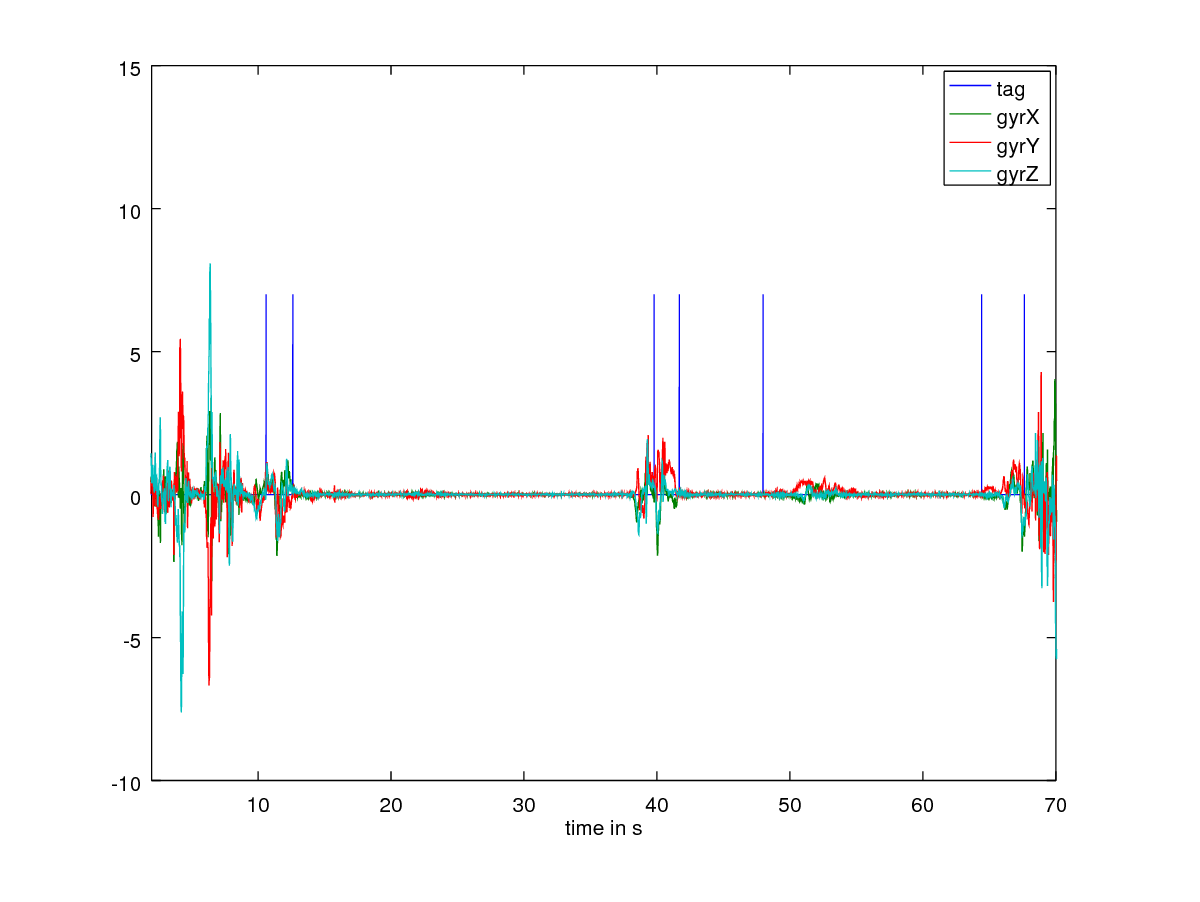
\includegraphics[width=.45\textwidth]{eleup12_g} &
		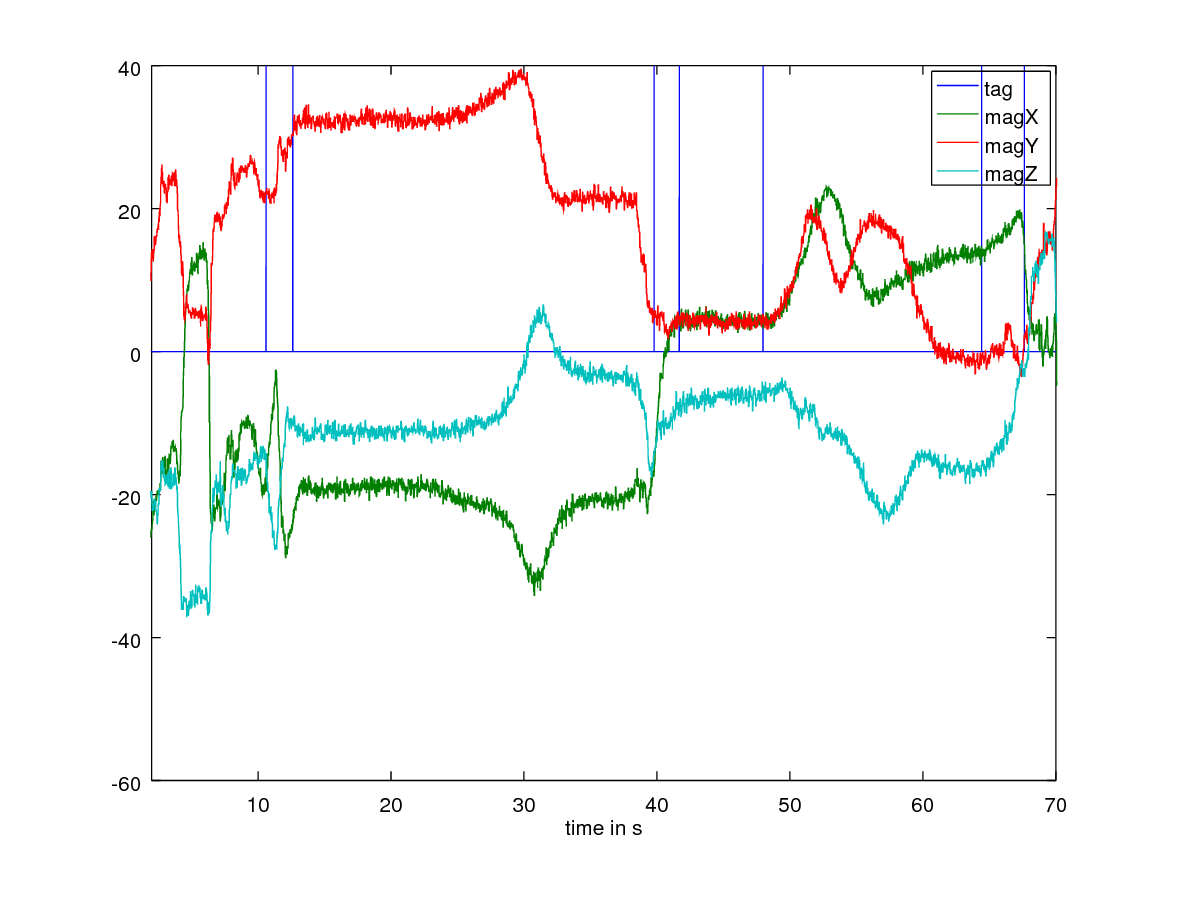
\includegraphics[width=.45\textwidth]{eleup12_m} 
		\\
		(c) & (d)

	\end{tabular}
	%
	\caption{Test case 2}
	\label{fig:Test_case_elevator_2}
\end{figure}


%%%----------------------------------------------------------
\section{Test case 3}
%%%----------------------------------------------------------
Test case 3 in Fig.~\ref{fig:Test_case_elevator_3}
\begin{figure}
	\centering\small
	\setlength{\tabcolsep}{0mm}	% alle Spaltenränder auf 0mm
	\begin{tabular}{c@{\hspace{12mm}}c} % mittlerer Abstand = 12mm
		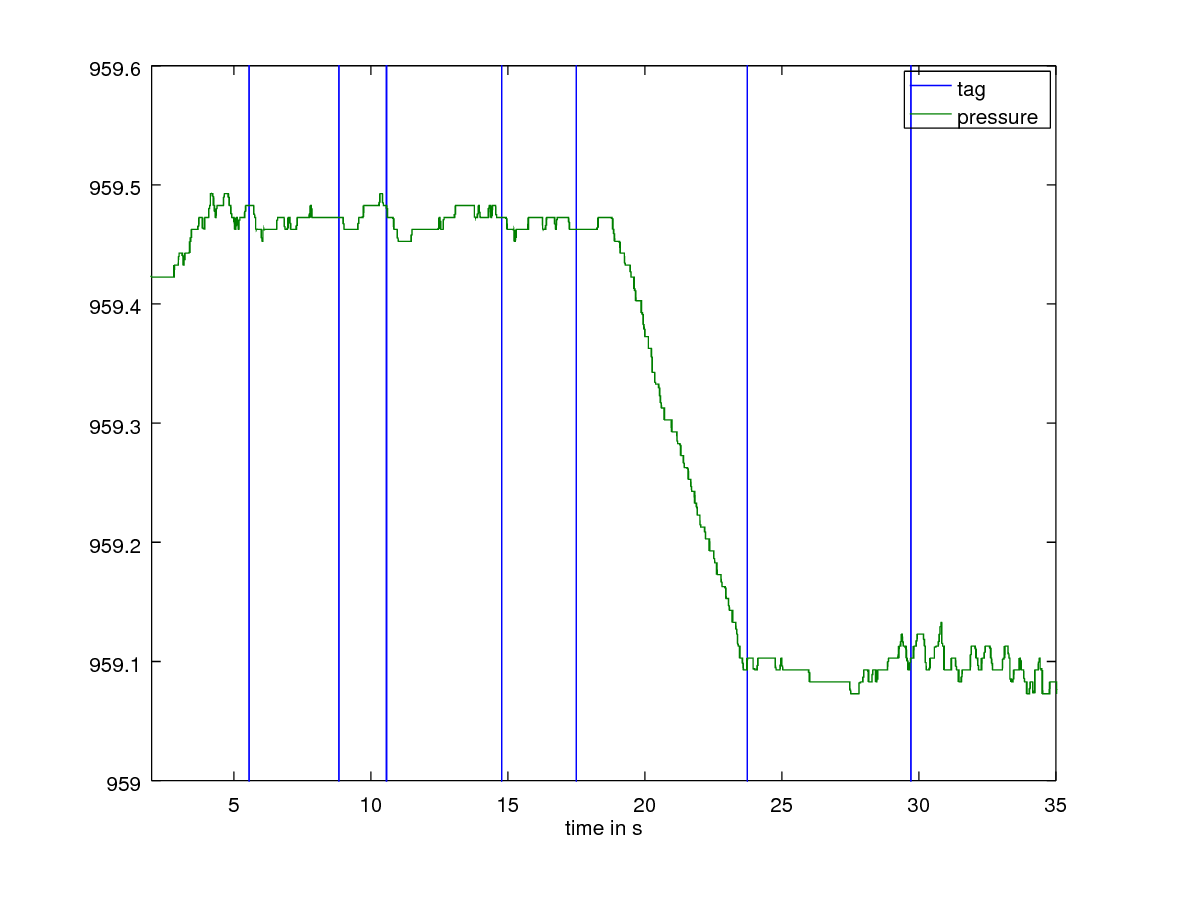
\includegraphics[width=.45\textwidth]{elevup8999puy_p} &
		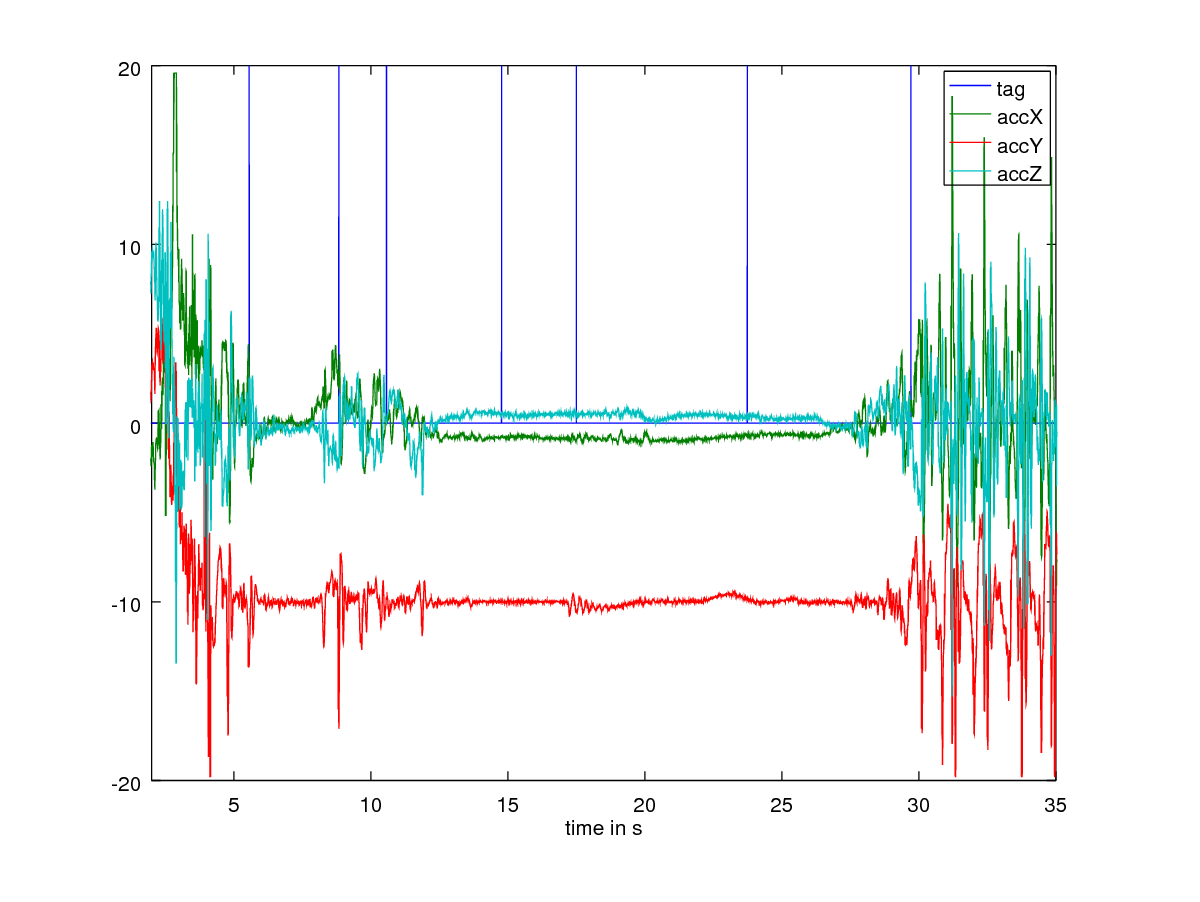
\includegraphics[width=.45\textwidth]{elevup8999puy_a} 
		\\
		(a) & (b)
		\\[4pt]	%vertical extra spacing (4 points)
		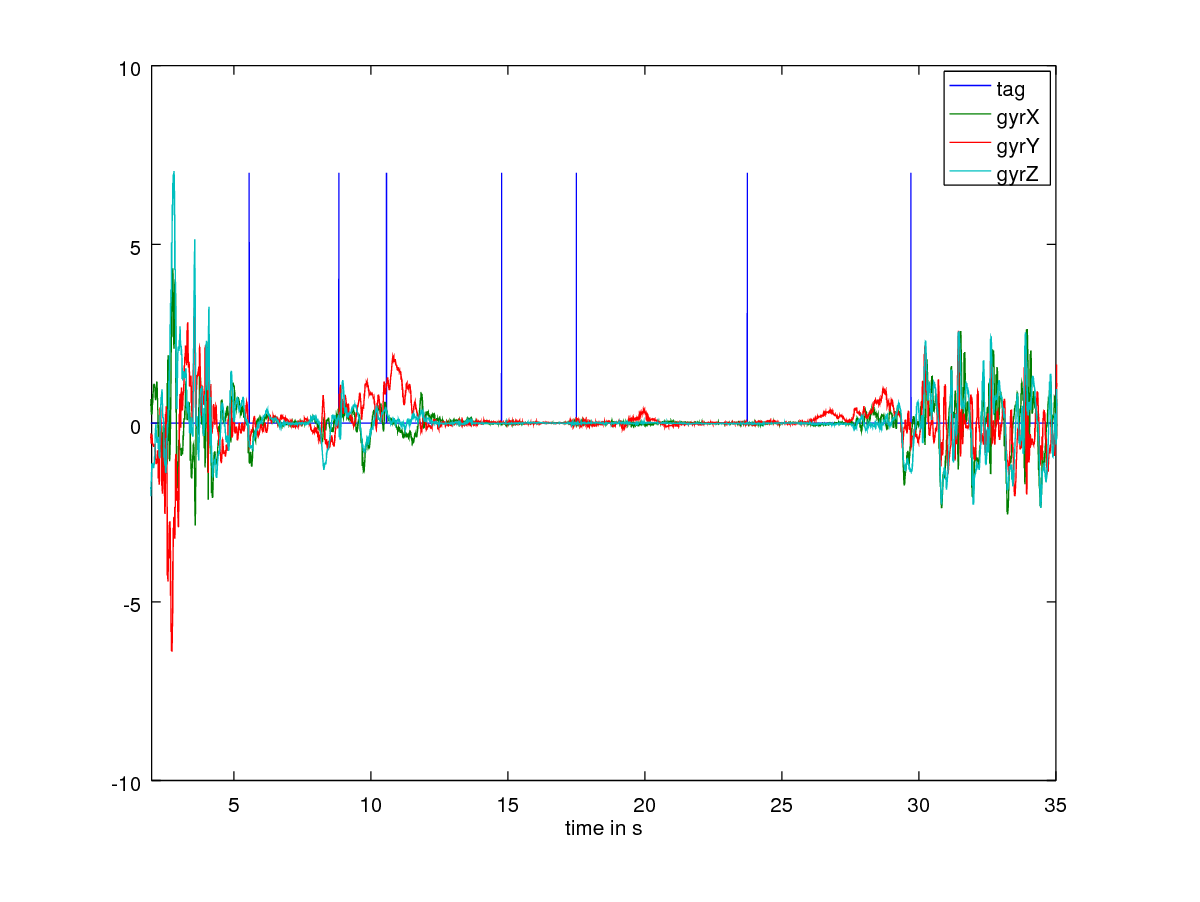
\includegraphics[width=.45\textwidth]{elevup8999puy_g} &
		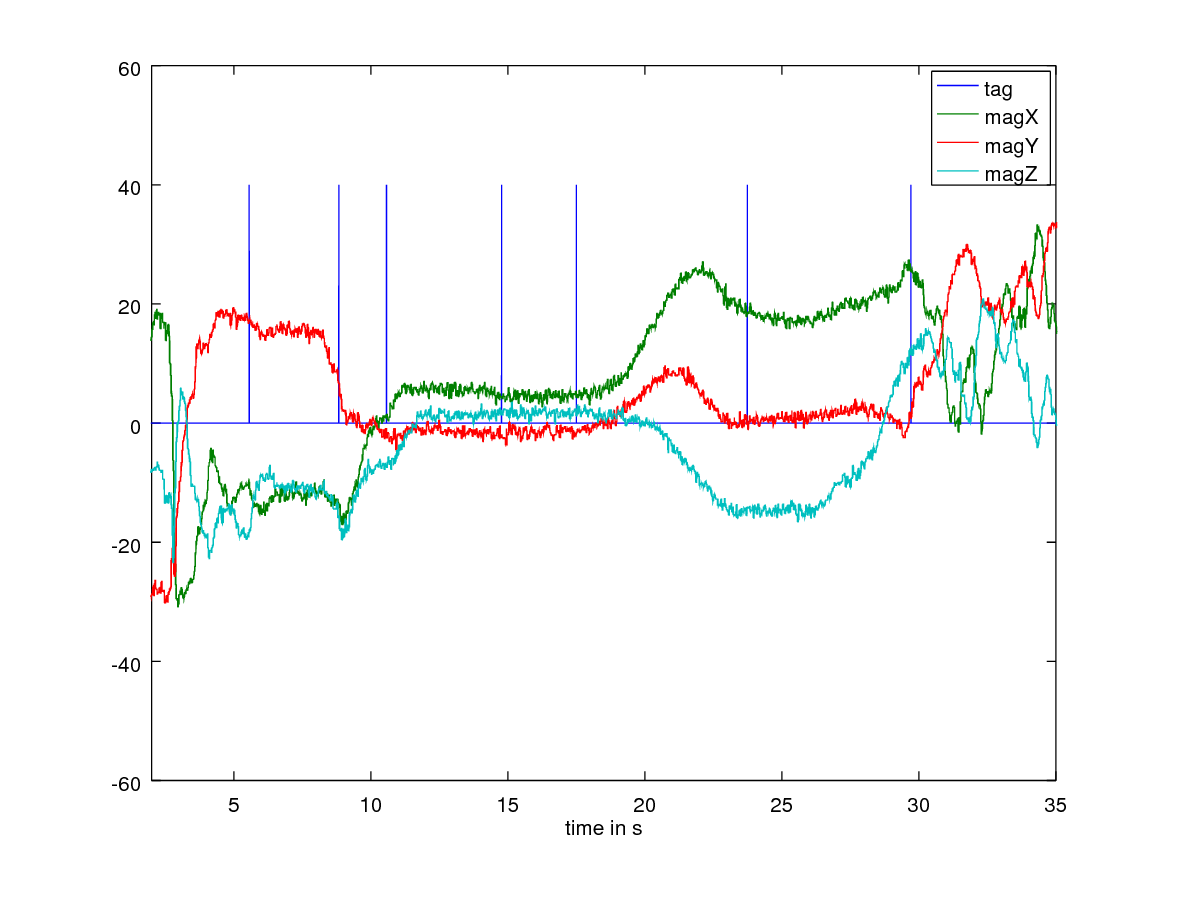
\includegraphics[width=.45\textwidth]{elevup8999puy_m} 
		\\
		(c) & (d)

	\end{tabular}
	%
	\caption{Test case 3}
	\label{fig:Test_case_elevator_3}
\end{figure}

%%%----------------------------------------------------------
\section{Test case 4}
%%%----------------------------------------------------------
Test case 4 in Fig.~\ref{fig:Test_case_elevator_4}
\begin{figure}
	\centering\small
	\setlength{\tabcolsep}{0mm}	% alle Spaltenränder auf 0mm
	\begin{tabular}{c@{\hspace{12mm}}c} % mittlerer Abstand = 12mm
		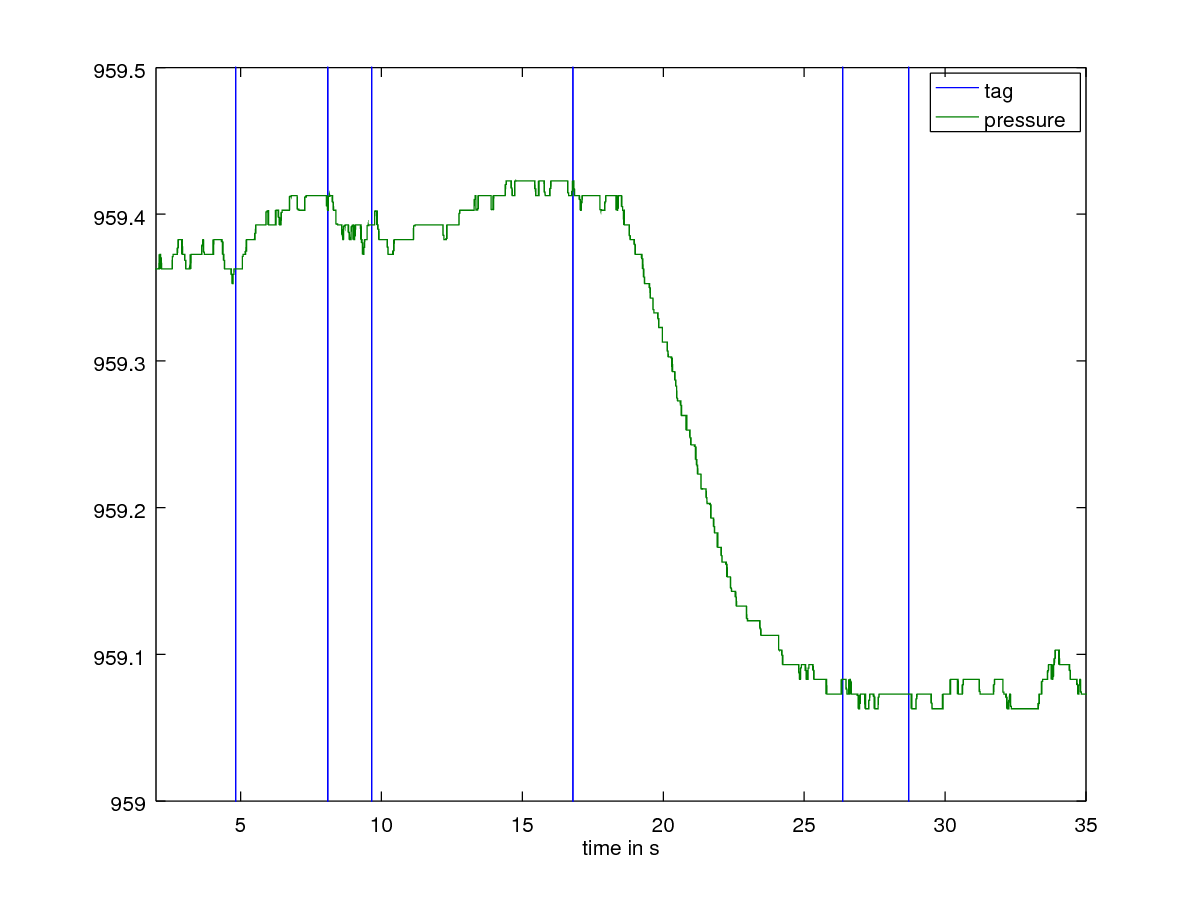
\includegraphics[width=.45\textwidth]{elevup55899_p} &
		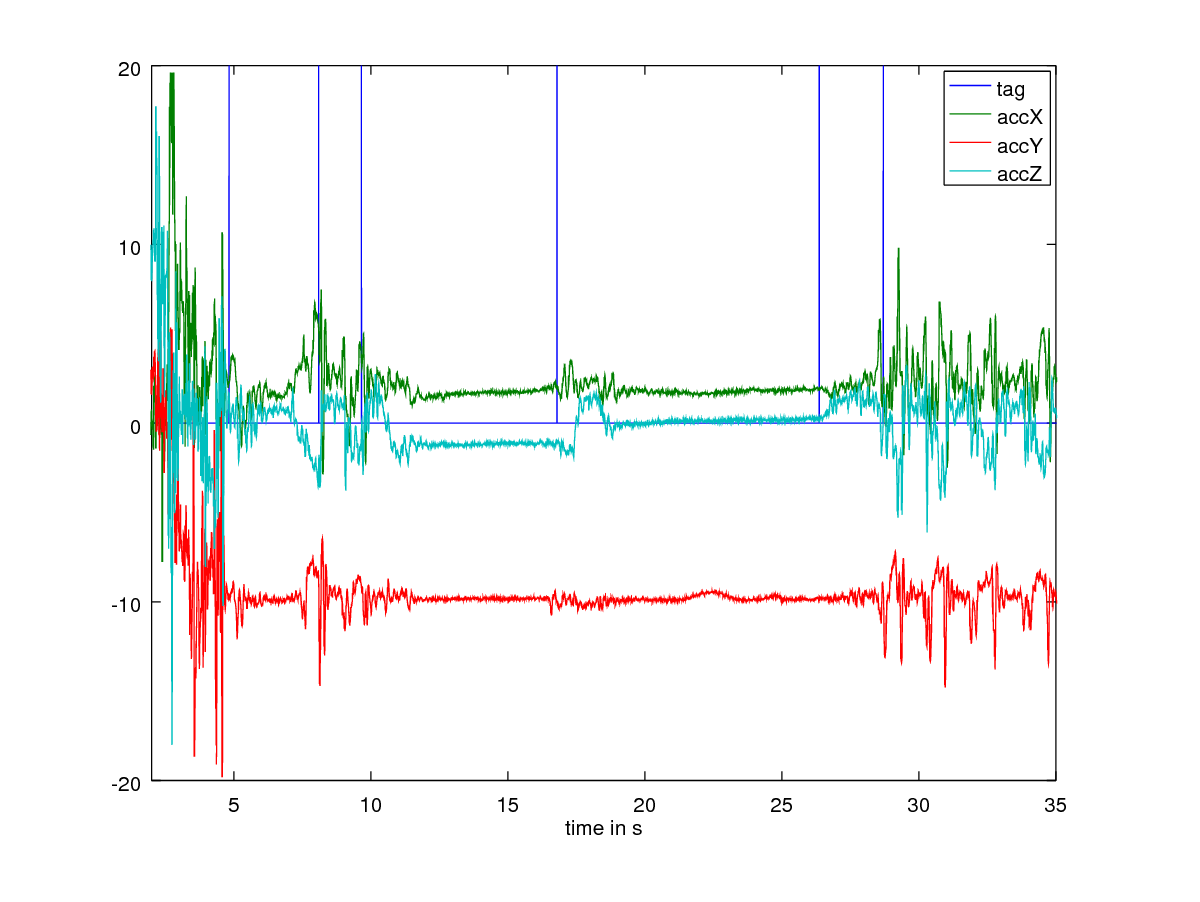
\includegraphics[width=.45\textwidth]{elevup55899_a} 
		\\
		(a) & (b)
		\\[4pt]	%vertical extra spacing (4 points)
		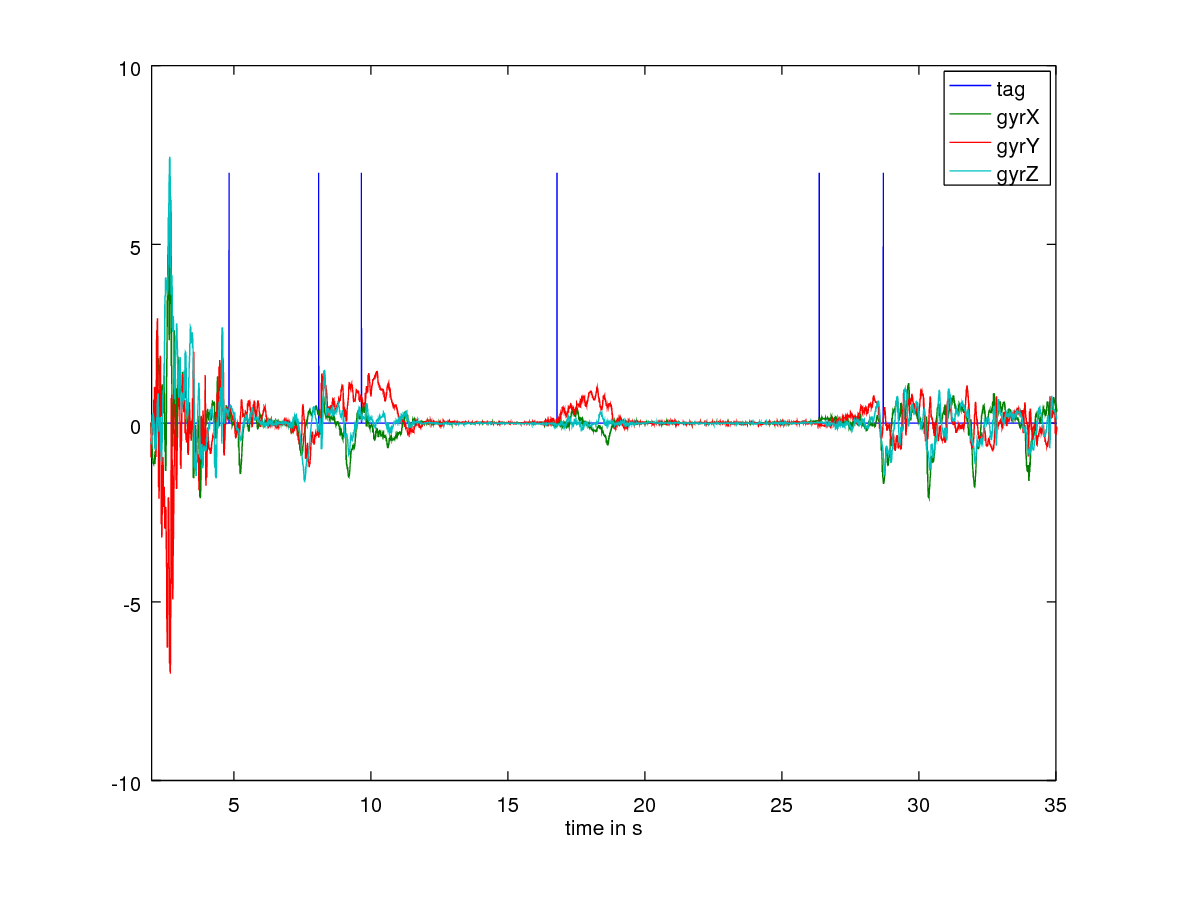
\includegraphics[width=.45\textwidth]{elevup55899_g} &
		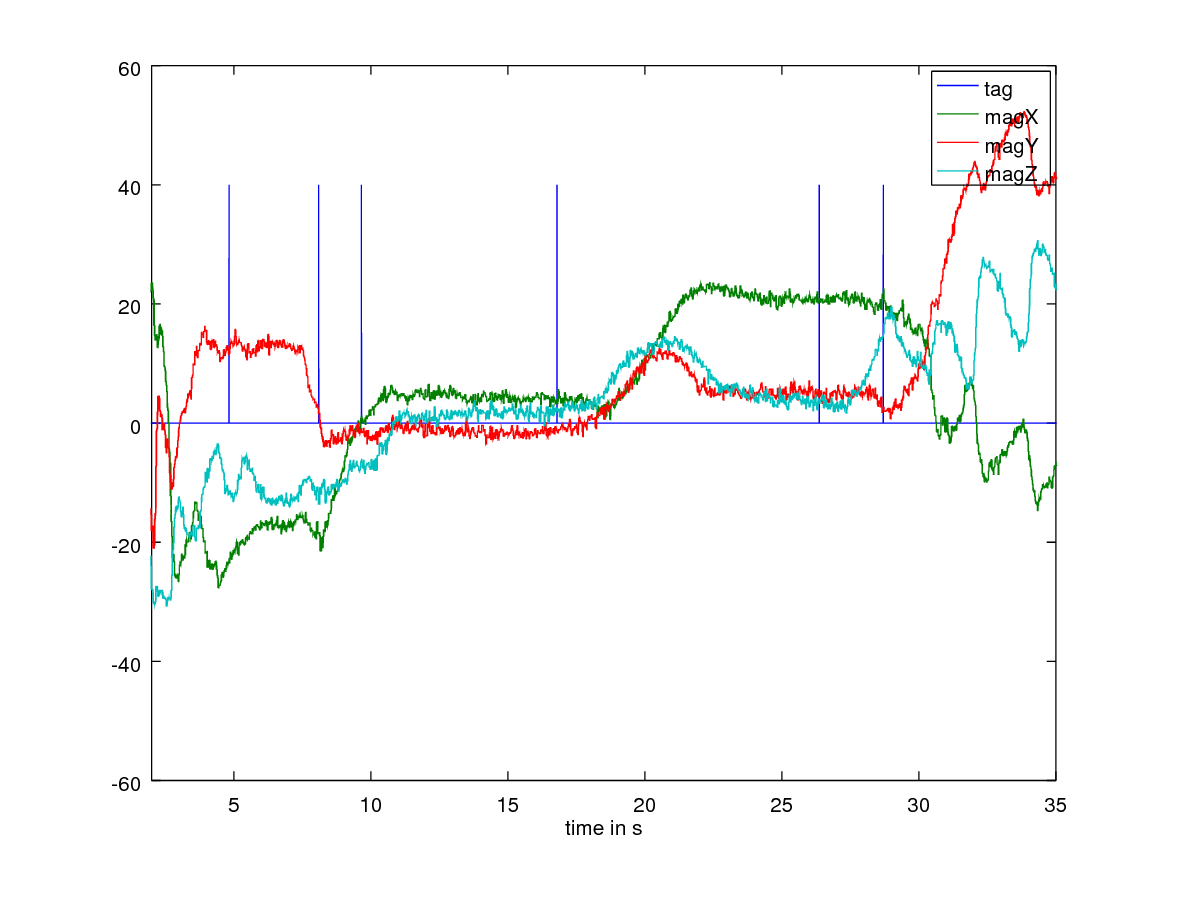
\includegraphics[width=.45\textwidth]{elevup55899_m} 
		\\
		(c) & (d)

	\end{tabular}
	%
	\caption{Test case 4}
	\label{fig:Test_case_elevator_4}
\end{figure}

%%%----------------------------------------------------------
\section{Test case 5}
%%%----------------------------------------------------------
Test case 5 in Fig.~\ref{fig:Test_case_elevator_5}
\begin{figure}
	\centering\small
	\setlength{\tabcolsep}{0mm}	% alle Spaltenränder auf 0mm
	\begin{tabular}{c@{\hspace{12mm}}c} % mittlerer Abstand = 12mm
		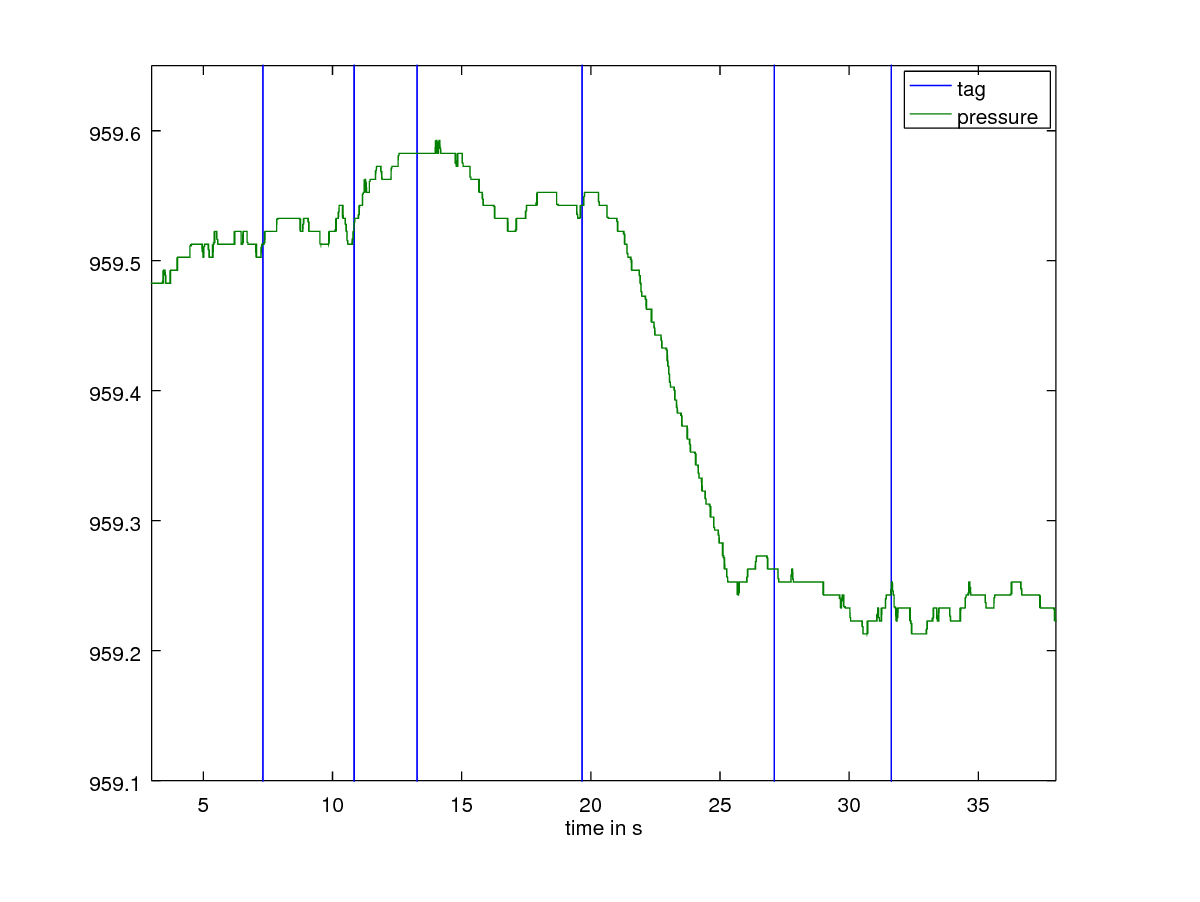
\includegraphics[width=.45\textwidth]{elevupc12_p} &
		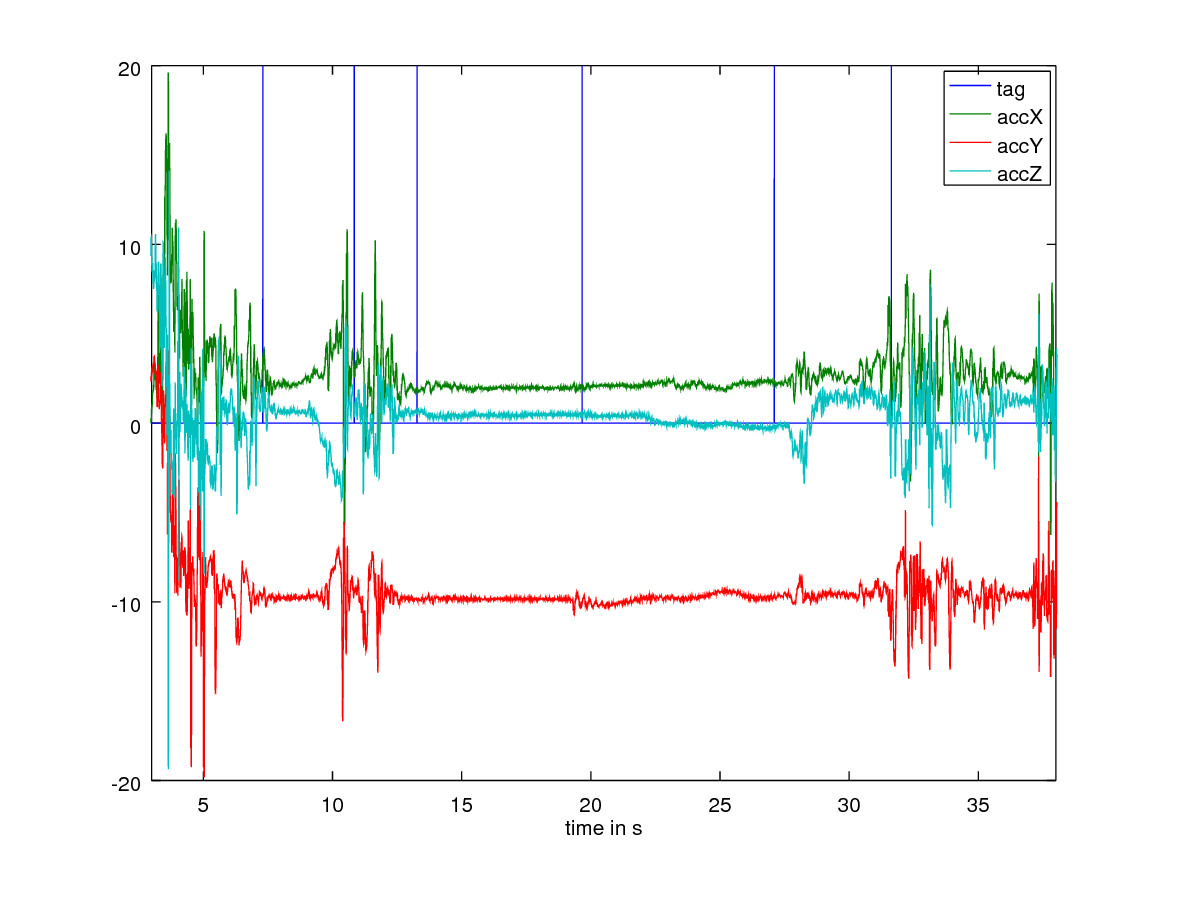
\includegraphics[width=.45\textwidth]{elevupc12_a} 
		\\
		(a) & (b)
		\\[4pt]	%vertical extra spacing (4 points)
		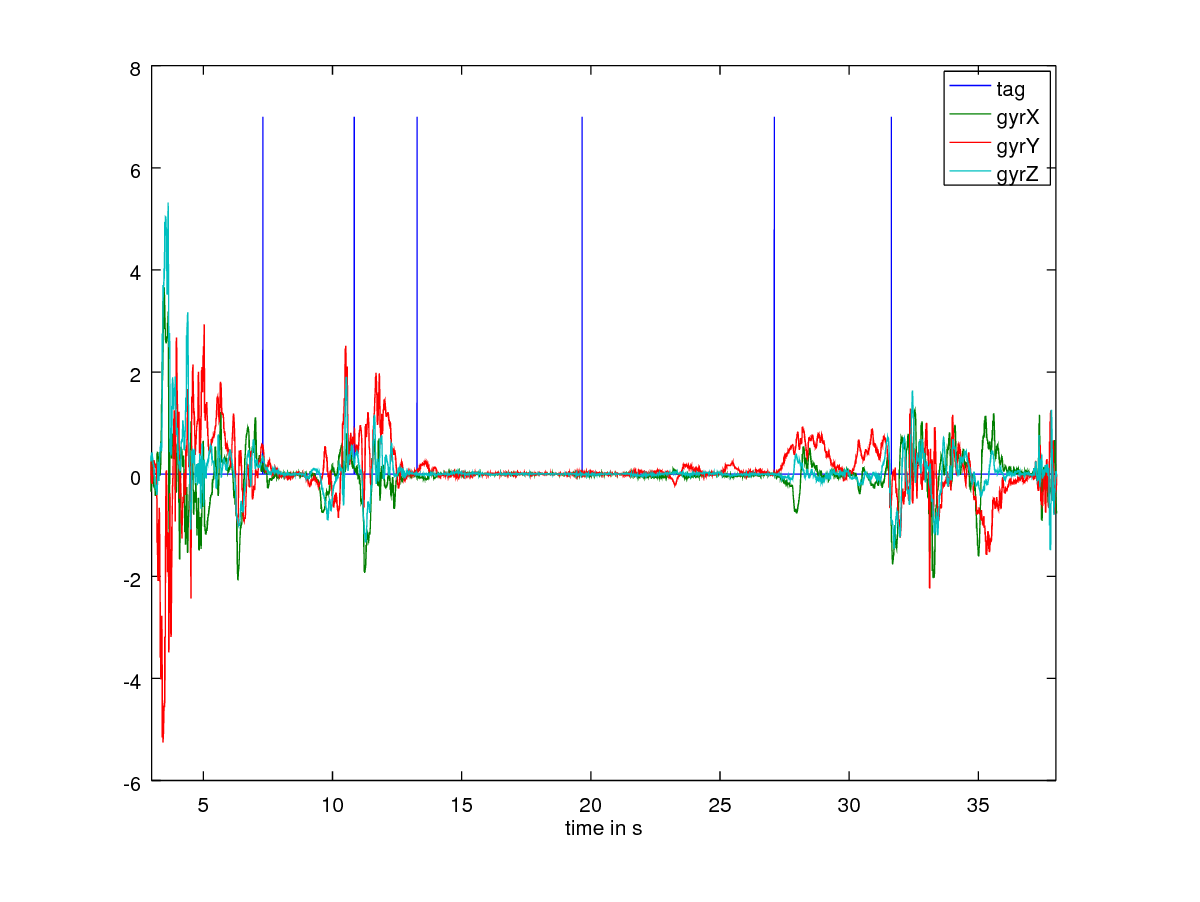
\includegraphics[width=.45\textwidth]{elevupc12_g} &
		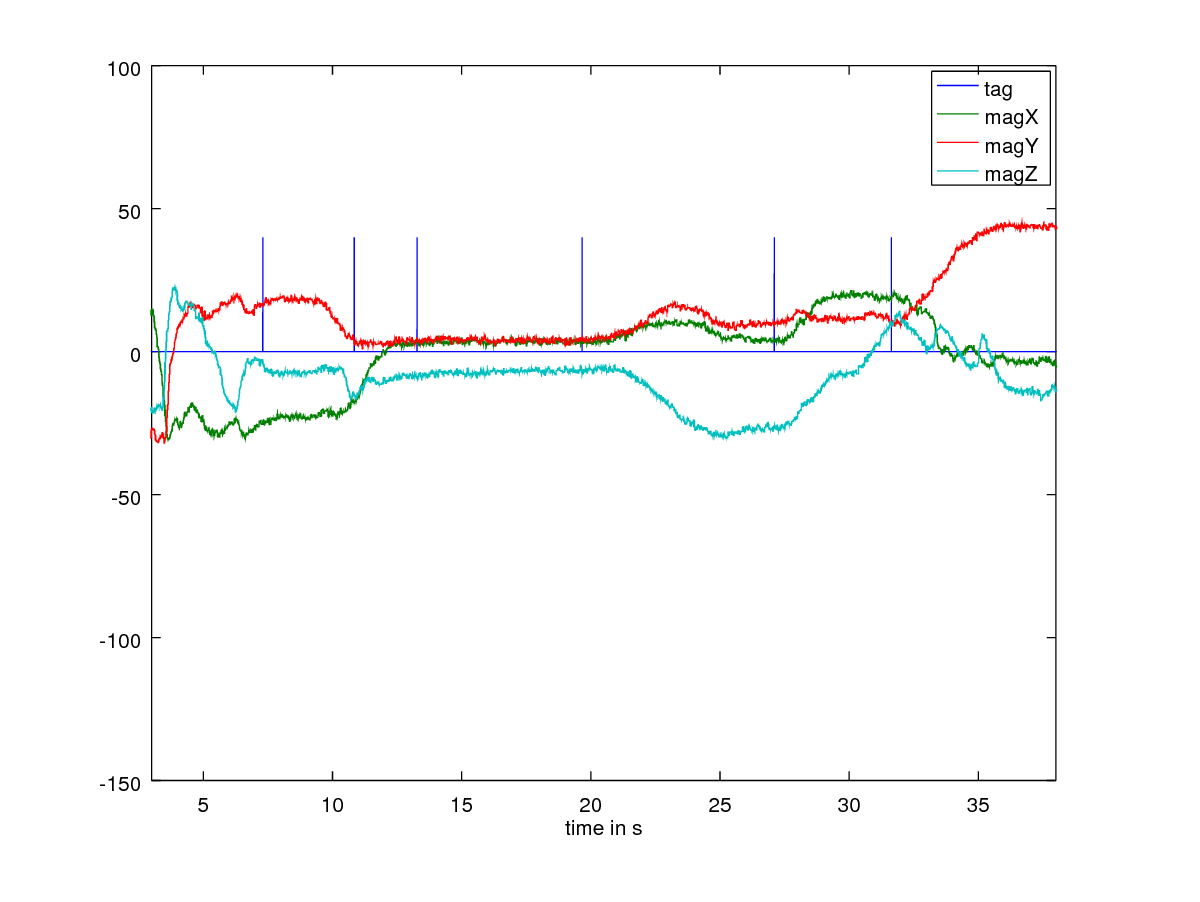
\includegraphics[width=.45\textwidth]{elevupc12_m} 
		\\
		(c) & (d)

	\end{tabular}
	%
	\caption{Test case 5}
	\label{fig:Test_case_elevator_5}
\end{figure}

%%%----------------------------------------------------------
\section{Test case 6}
%%%----------------------------------------------------------
Test case 6 in Fig.~\ref{fig:Test_case_elevator_6}
\begin{figure}
	\centering\small
	\setlength{\tabcolsep}{0mm}	% alle Spaltenränder auf 0mm
	\begin{tabular}{c@{\hspace{12mm}}c} % mittlerer Abstand = 12mm
		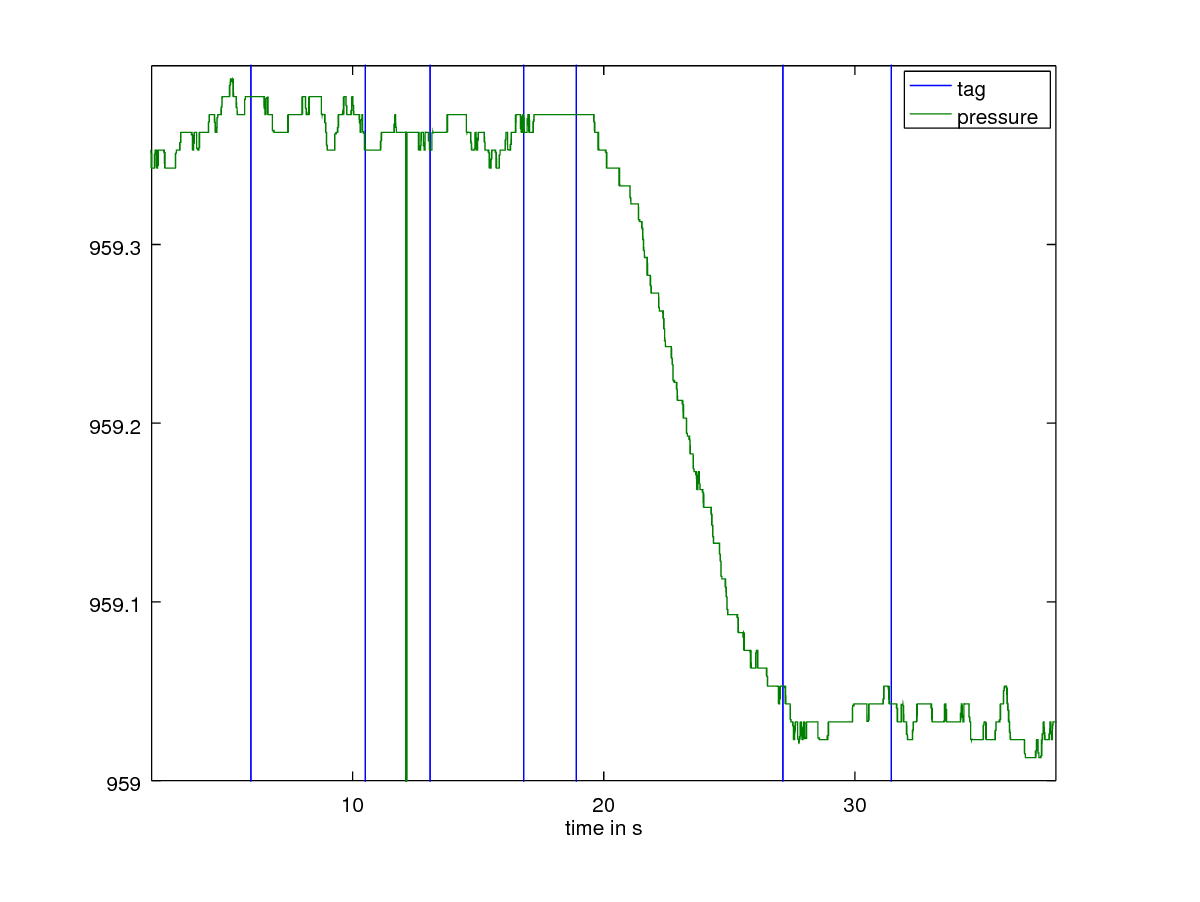
\includegraphics[width=.45\textwidth]{elevupkkiiuu45_p} &
		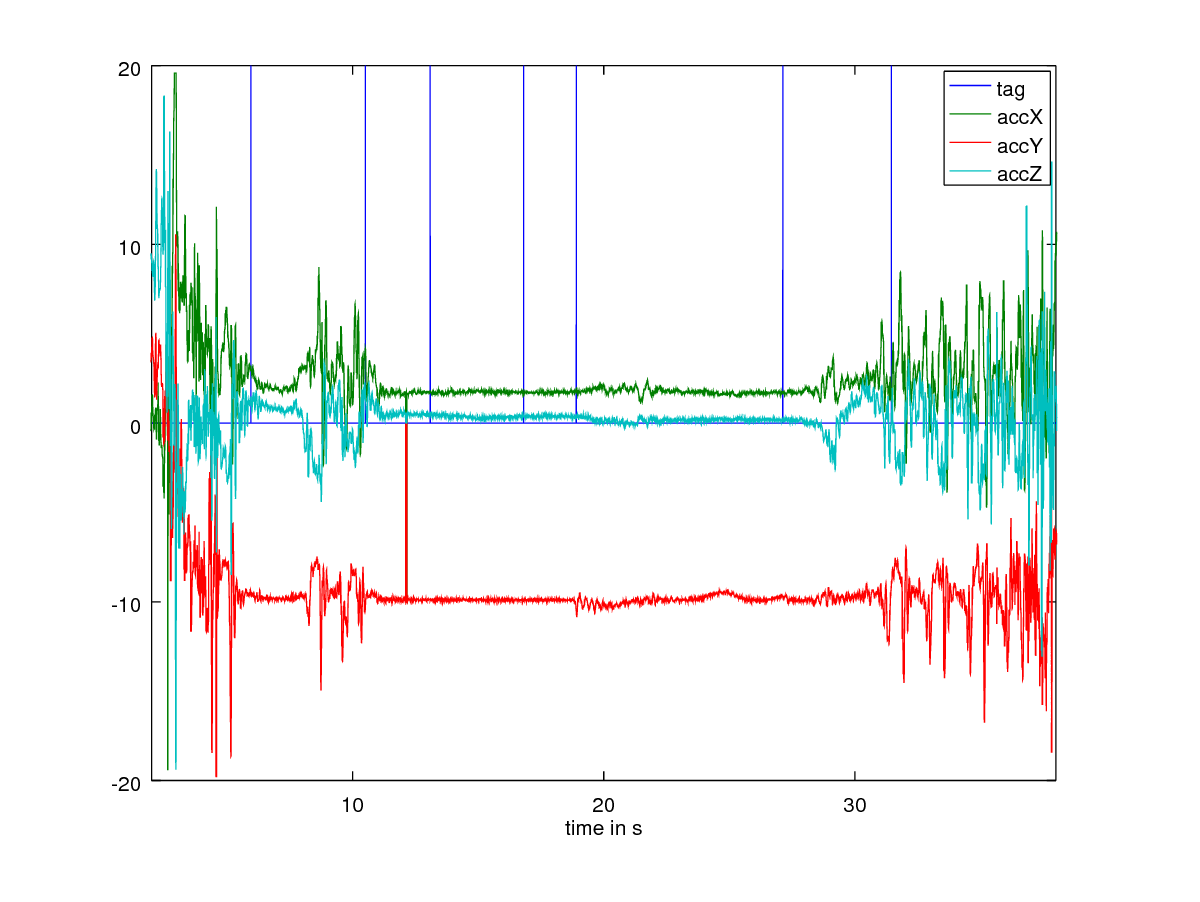
\includegraphics[width=.45\textwidth]{elevupkkiiuu45_a} 
		\\
		(a) & (b)
		\\[4pt]	%vertical extra spacing (4 points)
		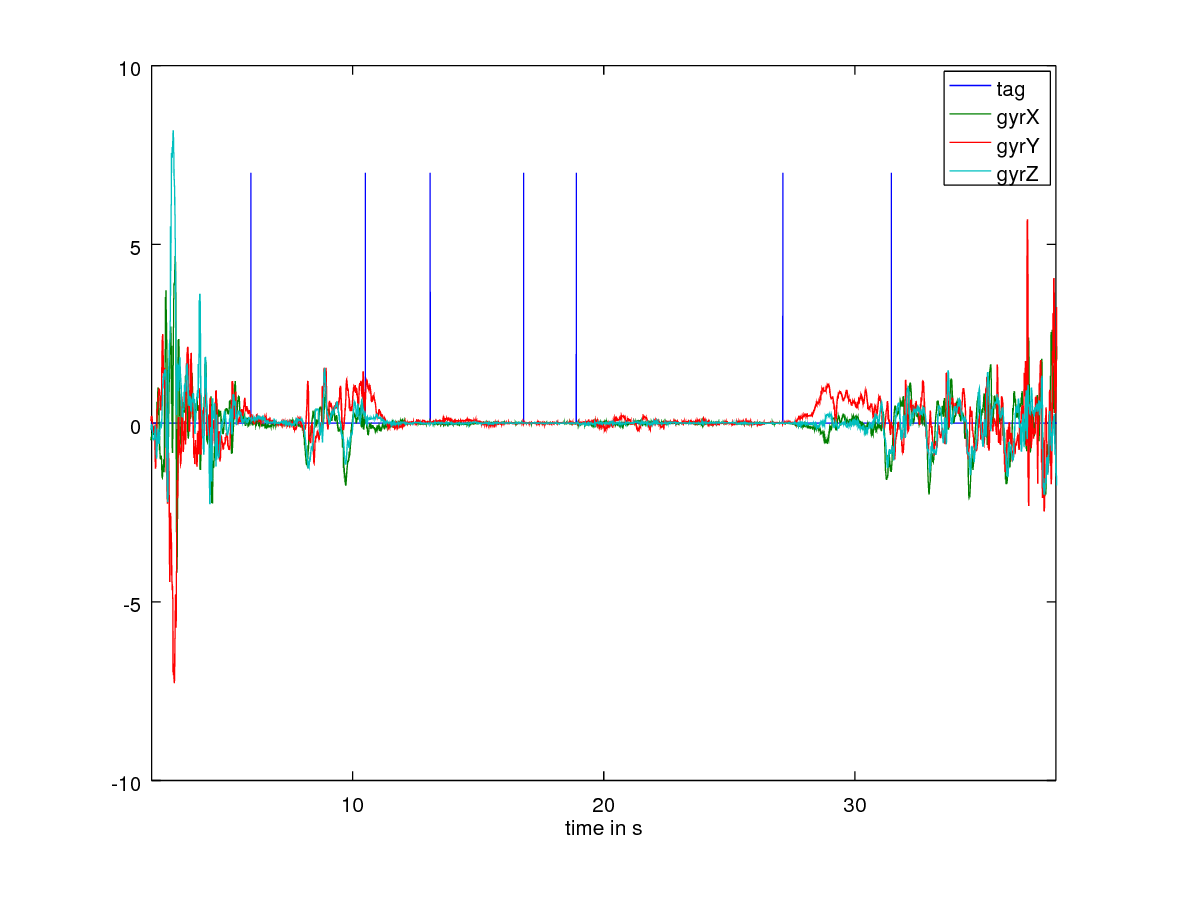
\includegraphics[width=.45\textwidth]{elevupkkiiuu45_g} &
		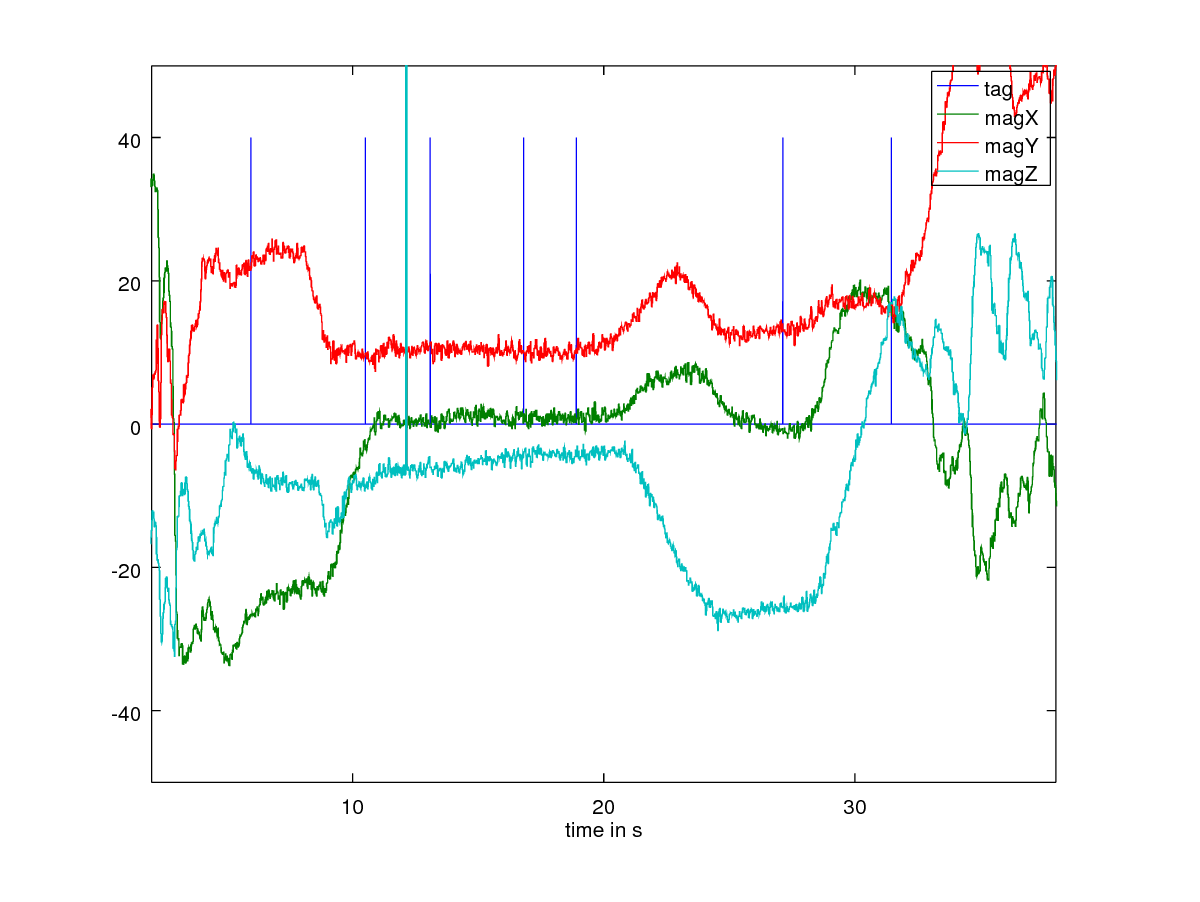
\includegraphics[width=.45\textwidth]{elevupkkiiuu45_m} 
		\\
		(c) & (d)

	\end{tabular}
	%
	\caption{Test case 6}
	\label{fig:Test_case_elevator_6}
\end{figure}


%%%----------------------------------------------------------
\section{Test case 7}
%%%----------------------------------------------------------
Test case 7 in Fig.~\ref{fig:Test_case_elevator_7}
\begin{figure}
	\centering\small
	\setlength{\tabcolsep}{0mm}	% alle Spaltenränder auf 0mm
	\begin{tabular}{c@{\hspace{12mm}}c} % mittlerer Abstand = 12mm
		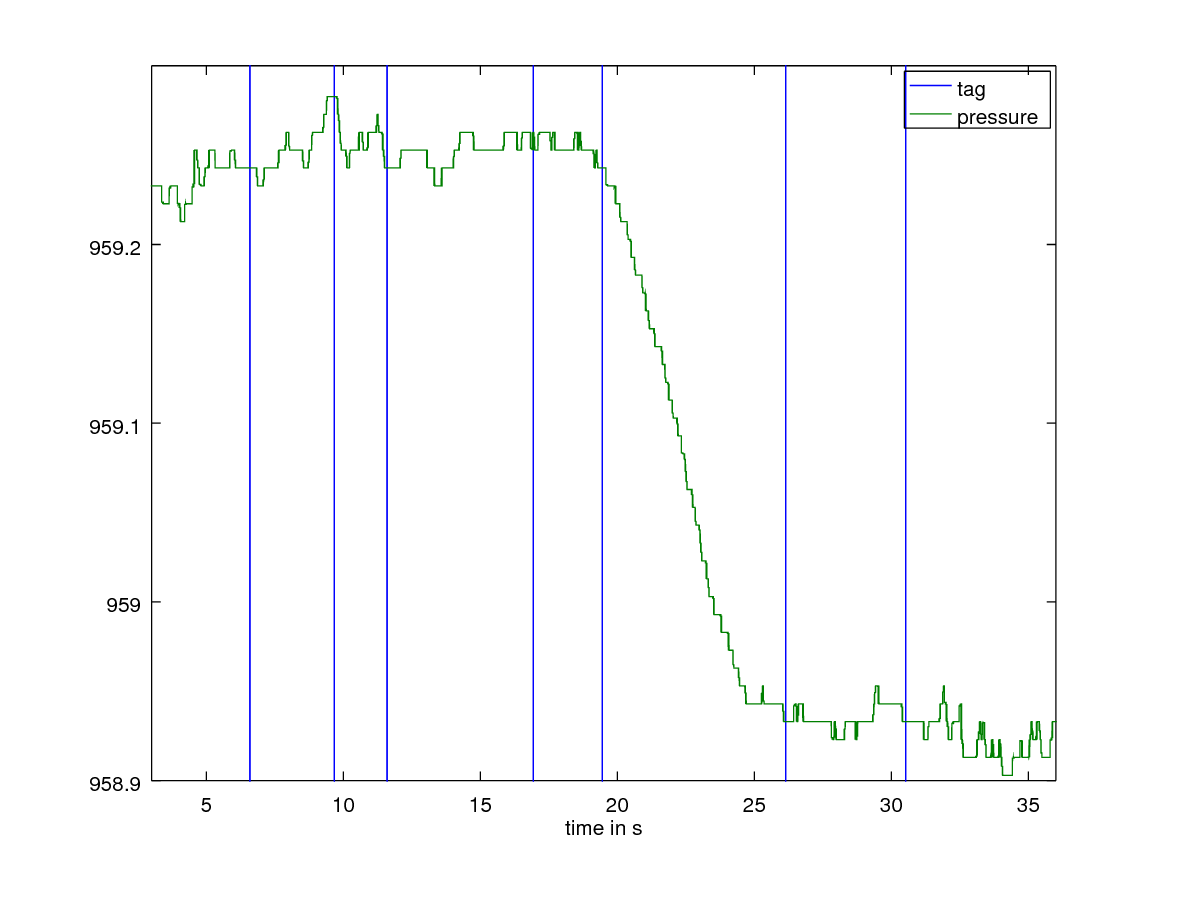
\includegraphics[width=.45\textwidth]{elevupmeganew7_p} &
		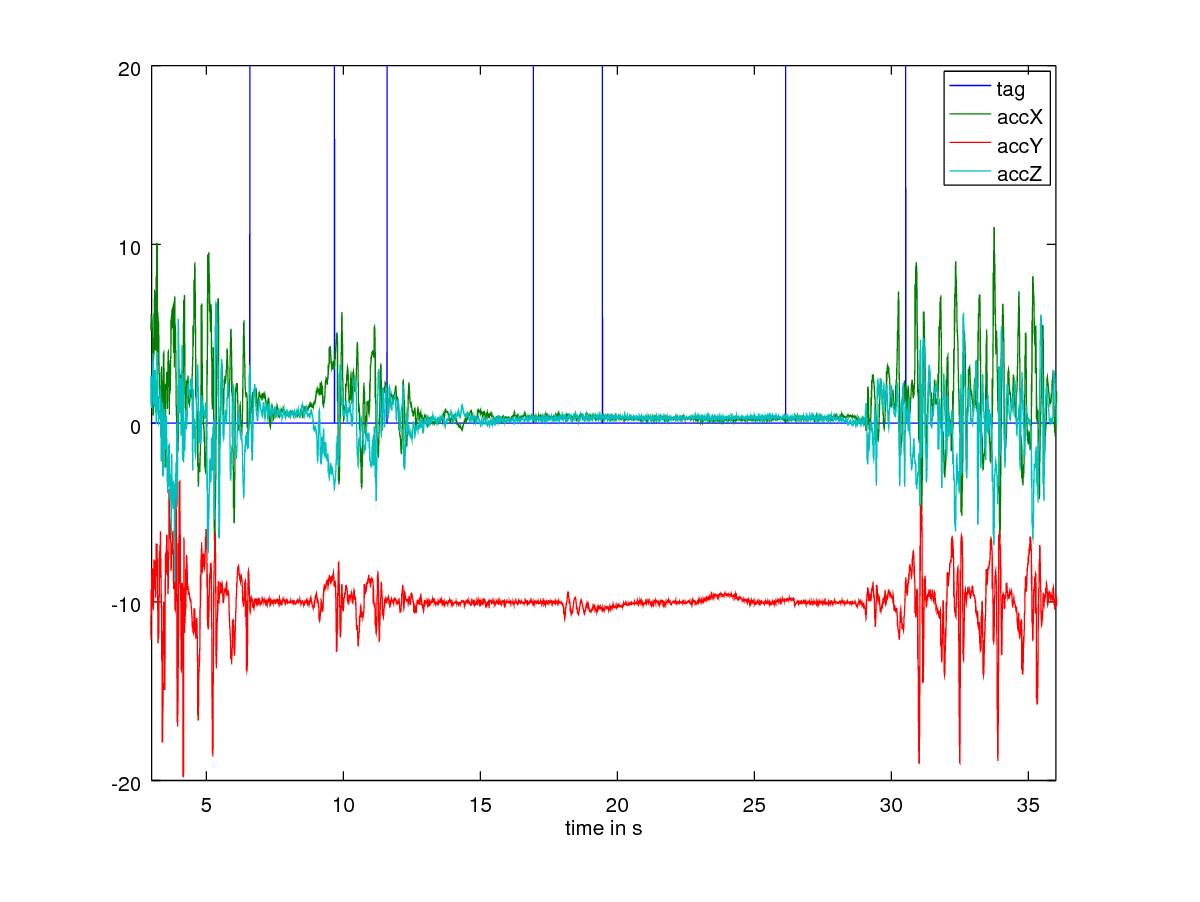
\includegraphics[width=.45\textwidth]{elevupmeganew7_a} 
		\\
		(a) & (b)
		\\[4pt]	%vertical extra spacing (4 points)
		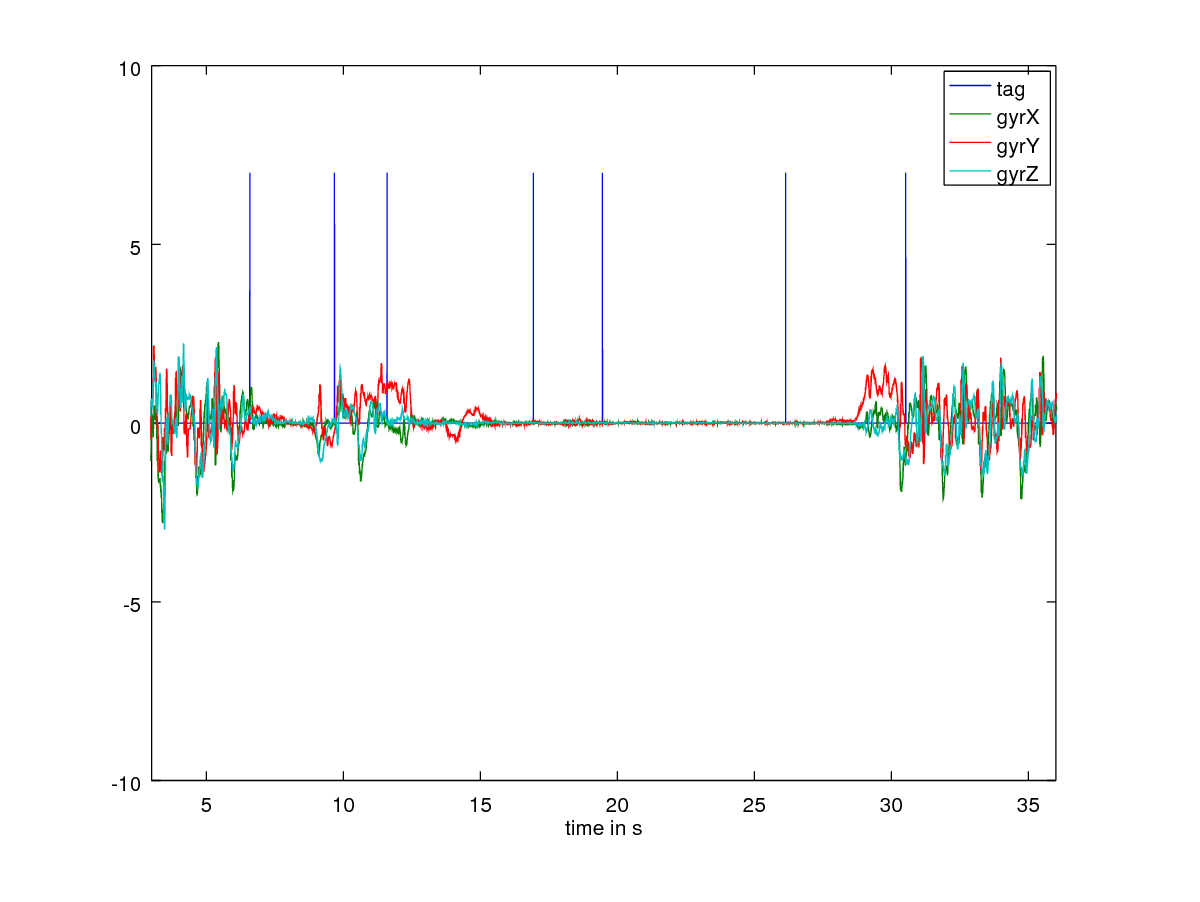
\includegraphics[width=.45\textwidth]{elevupmeganew7_g} &
		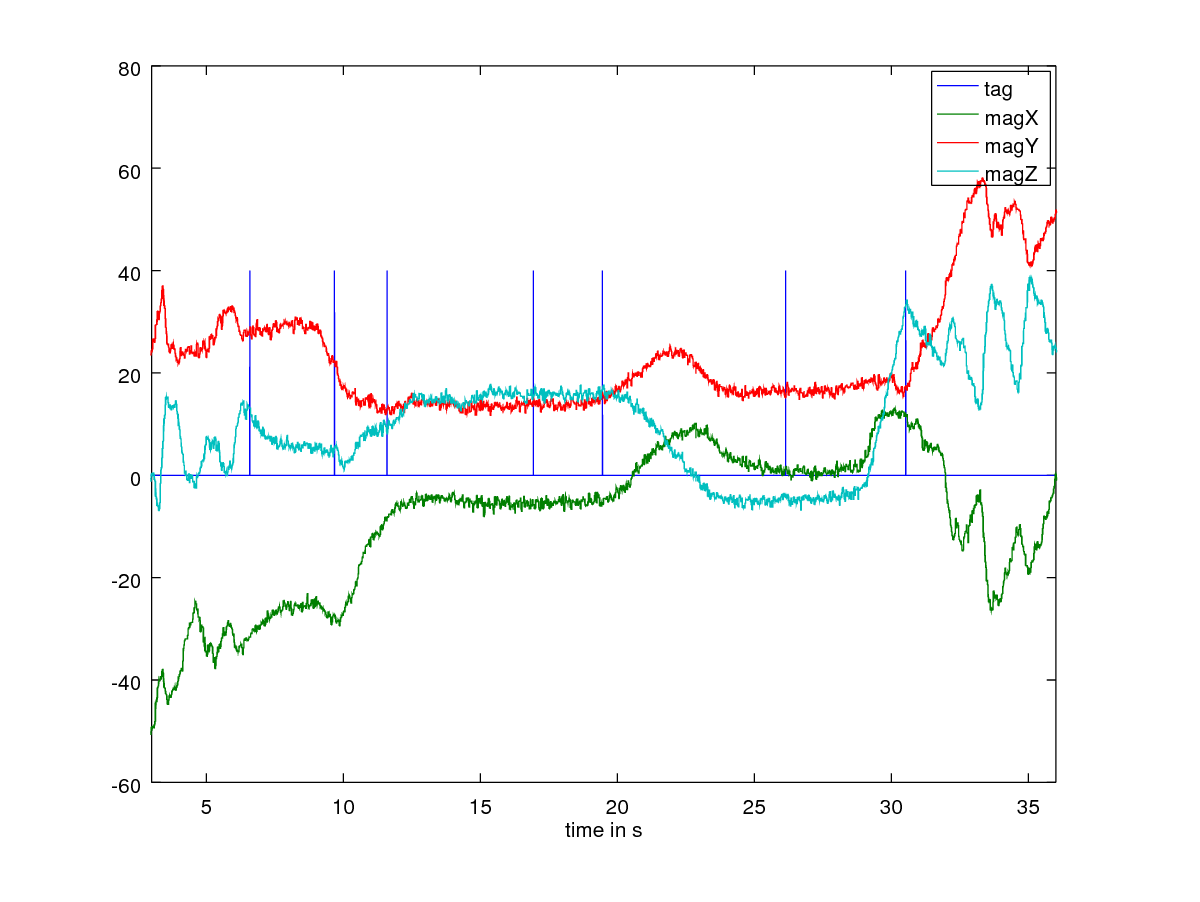
\includegraphics[width=.45\textwidth]{elevupmeganew7_m} 
		\\
		(c) & (d)

	\end{tabular}
	%
	\caption{Test case 7}
	\label{fig:Test_case_elevator_7}
\end{figure}


%%%----------------------------------------------------------
\section{Test case 8}
%%%----------------------------------------------------------
Test case 8 in Fig.~\ref{fig:Test_case_elevator_8}
\begin{figure}
	\centering\small
	\setlength{\tabcolsep}{0mm}	% alle Spaltenränder auf 0mm
	\begin{tabular}{c@{\hspace{12mm}}c} % mittlerer Abstand = 12mm
		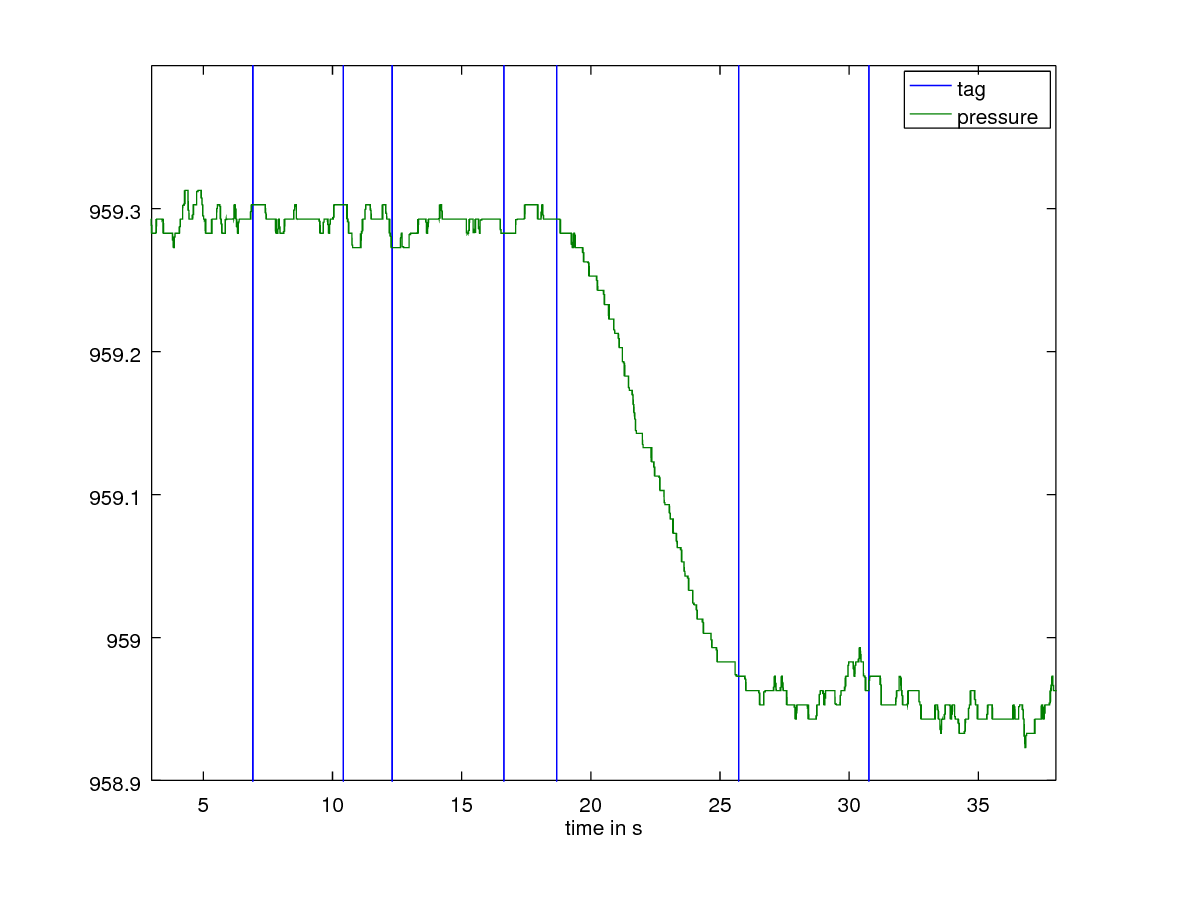
\includegraphics[width=.45\textwidth]{elevupnew558900_p} &
		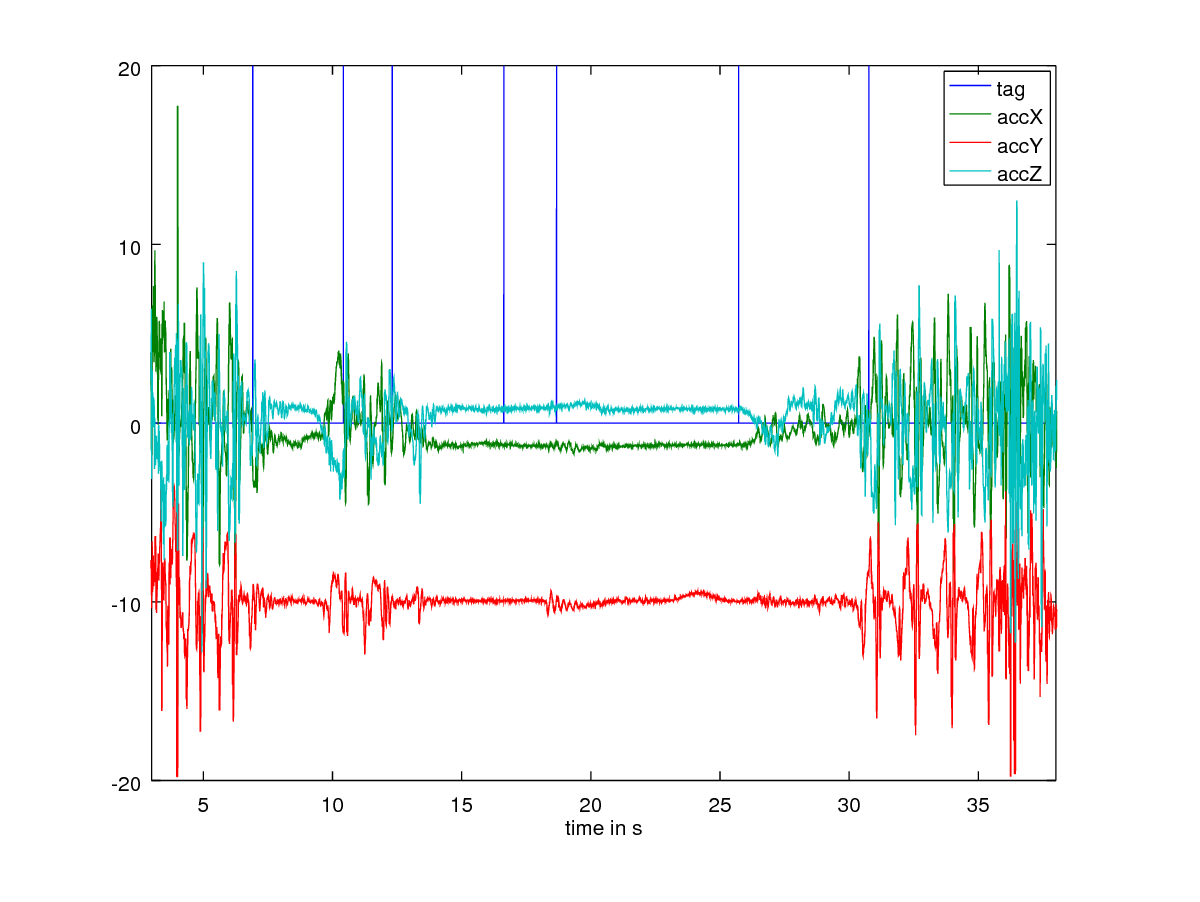
\includegraphics[width=.45\textwidth]{elevupnew558900_a} 
		\\
		(a) & (b)
		\\[4pt]	%vertical extra spacing (4 points)
		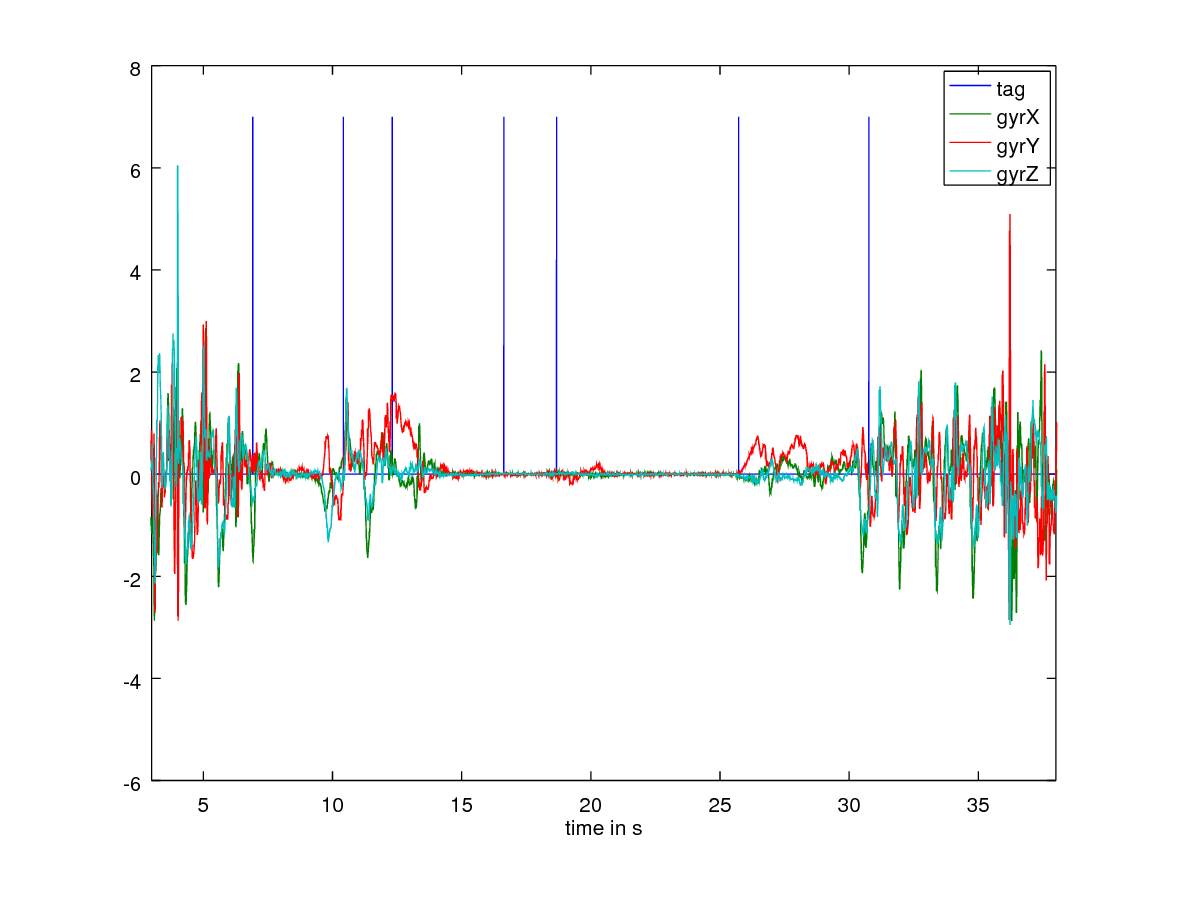
\includegraphics[width=.45\textwidth]{elevupnew558900_g} &
		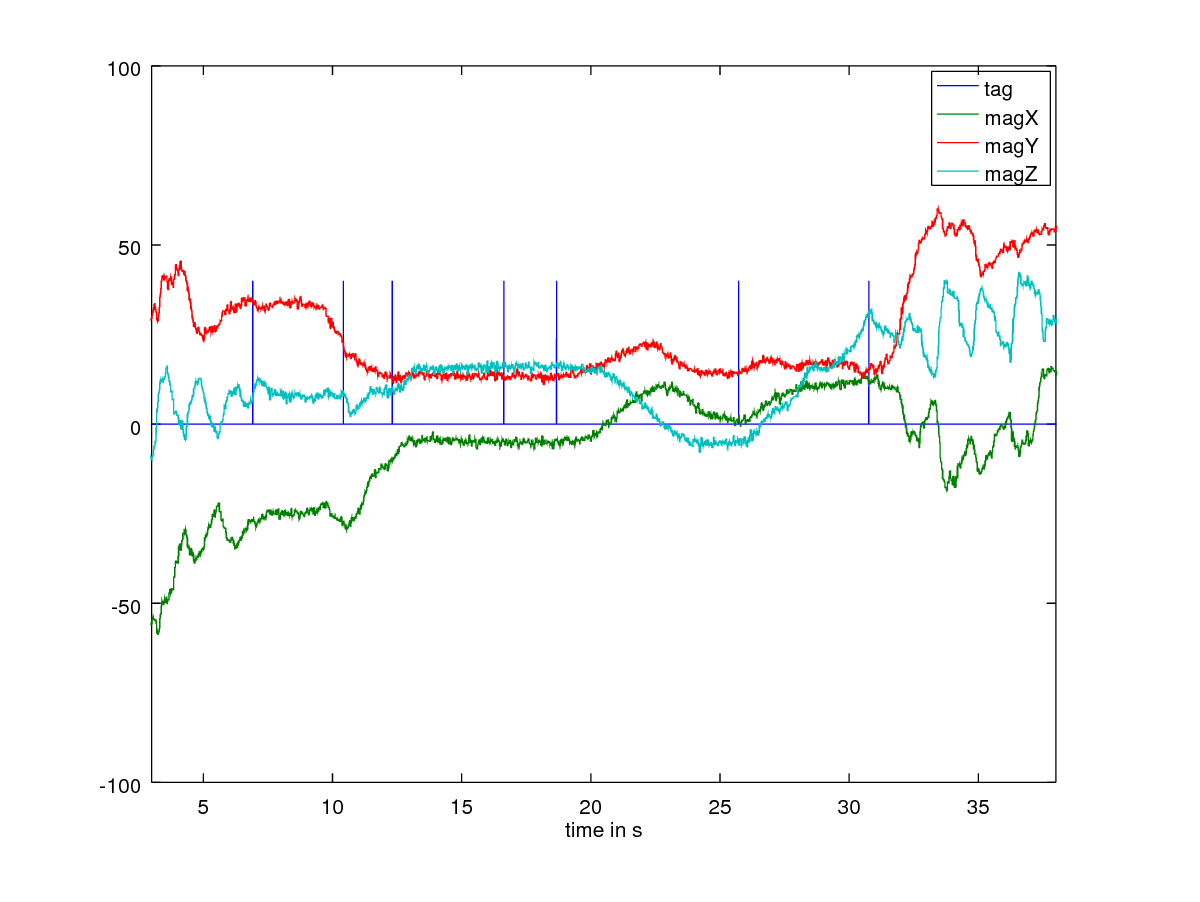
\includegraphics[width=.45\textwidth]{elevupnew558900_m} 
		\\
		(c) & (d)

	\end{tabular}
	%
	\caption{Test case 8}
	\label{fig:Test_case_elevator_8}
\end{figure}

%%%----------------------------------------------------------
\section{Test case 9}
%%%----------------------------------------------------------
Test case 9 in Fig.~\ref{fig:Test_case_elevator_9}
\begin{figure}
	\centering\small
	\setlength{\tabcolsep}{0mm}	% alle Spaltenränder auf 0mm
	\begin{tabular}{c@{\hspace{12mm}}c} % mittlerer Abstand = 12mm
		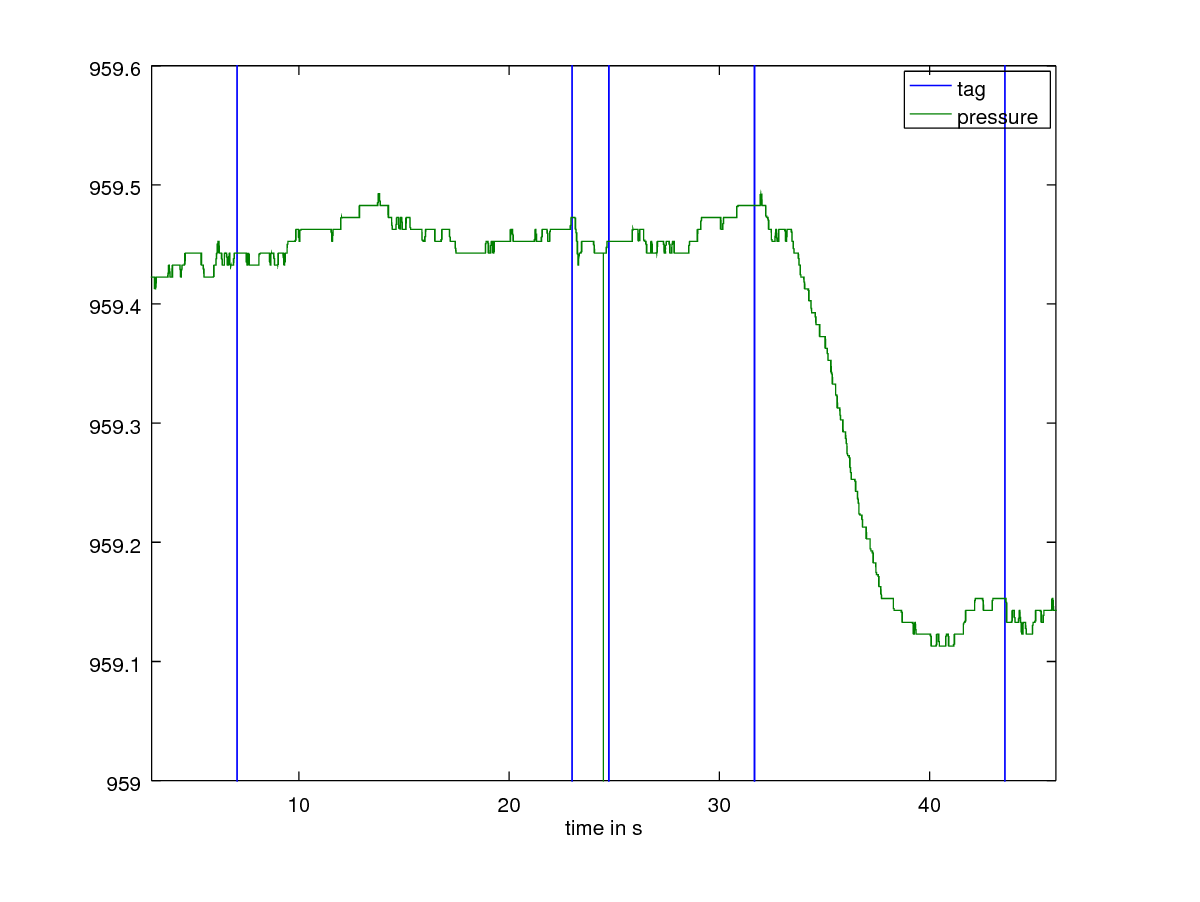
\includegraphics[width=.45\textwidth]{elevupuuu778_p} &
		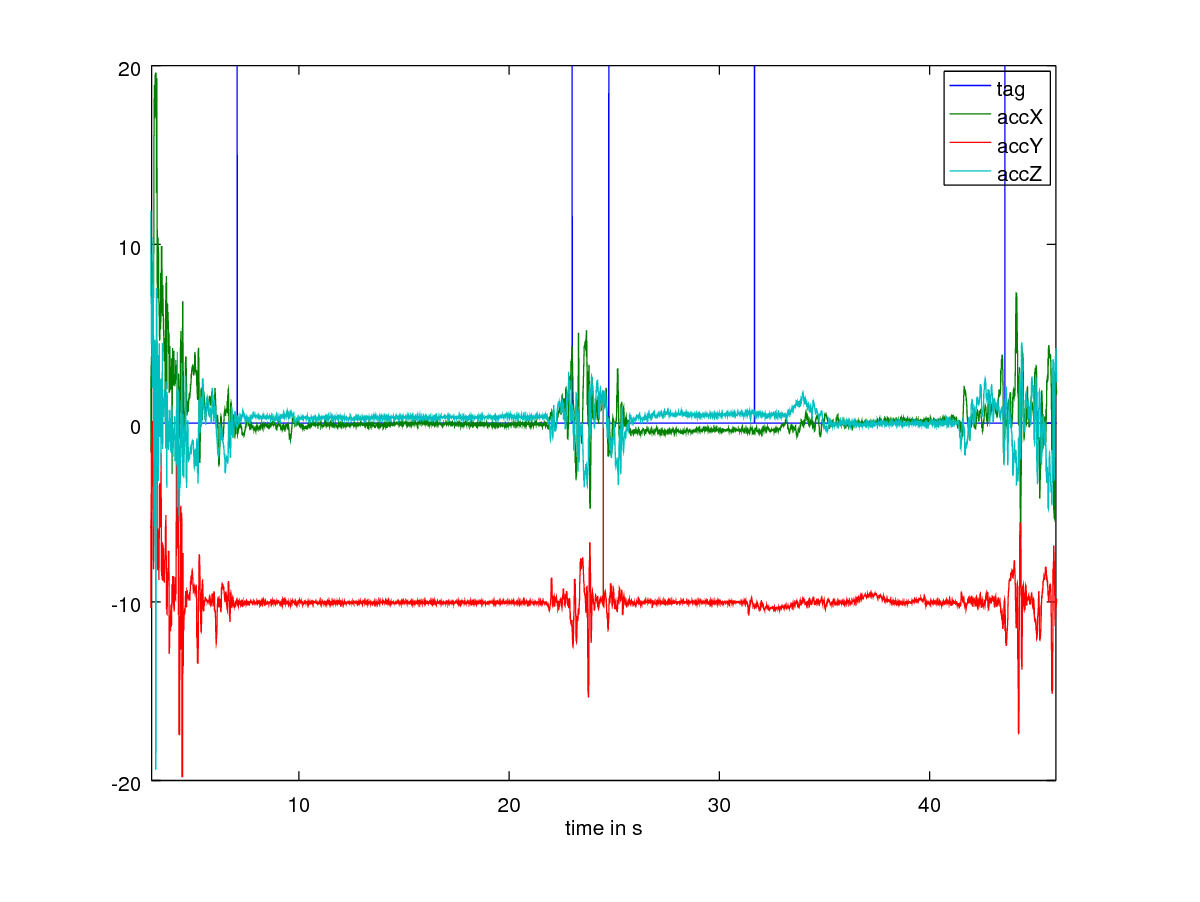
\includegraphics[width=.45\textwidth]{elevupuuu778_a} 
		\\
		(a) & (b)
		\\[4pt]	%vertical extra spacing (4 points)
		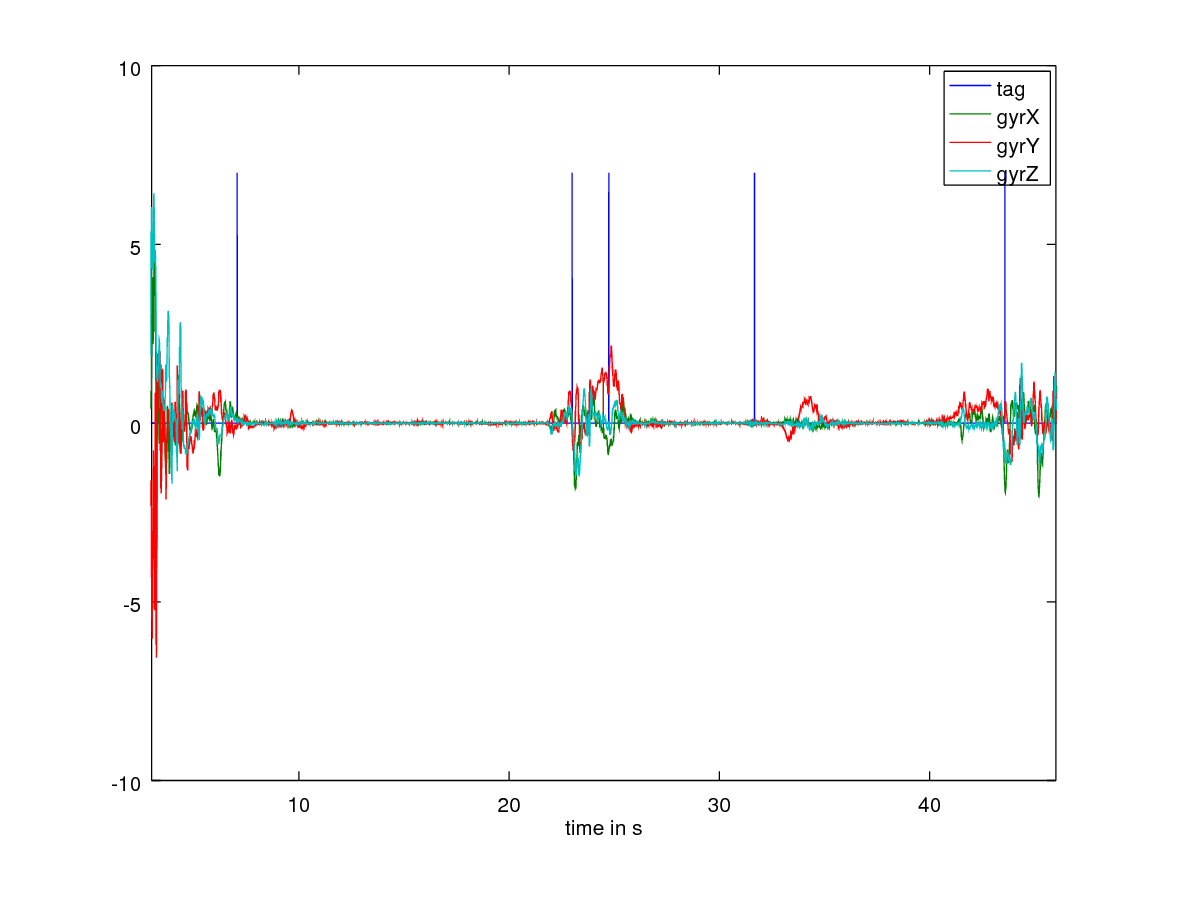
\includegraphics[width=.45\textwidth]{elevupuuu778_g} &
		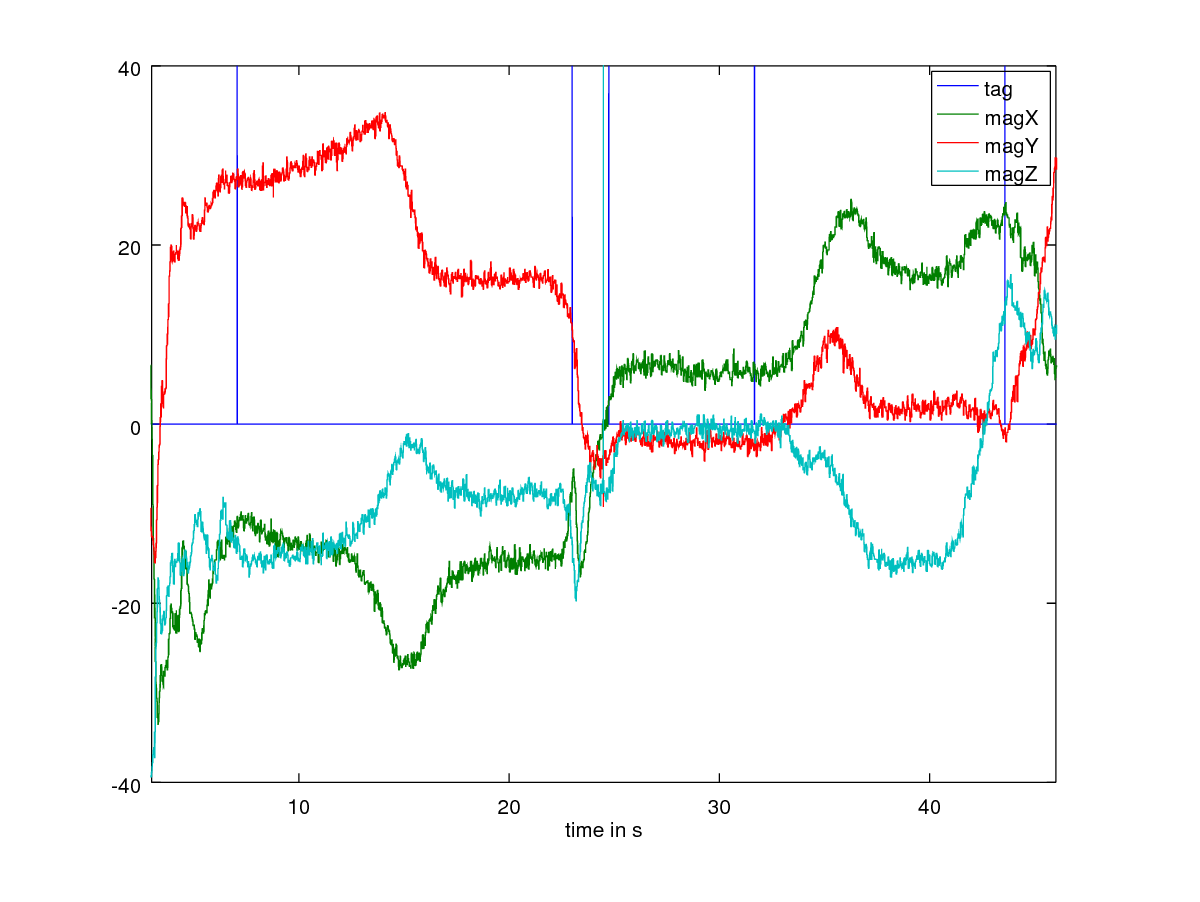
\includegraphics[width=.45\textwidth]{elevupuuu778_m} 
		\\
		(c) & (d)

	\end{tabular}
	%
	\caption{Test case 9}
	\label{fig:Test_case_elevator_9}
\end{figure}

%%%----------------------------------------------------------
\section{Test case 10}
%%%----------------------------------------------------------
Test case 10 in Fig.~\ref{fig:Test_case_elevator_10}
\begin{figure}
	\centering\small
	\setlength{\tabcolsep}{0mm}	% alle Spaltenränder auf 0mm
	\begin{tabular}{c@{\hspace{12mm}}c} % mittlerer Abstand = 12mm
		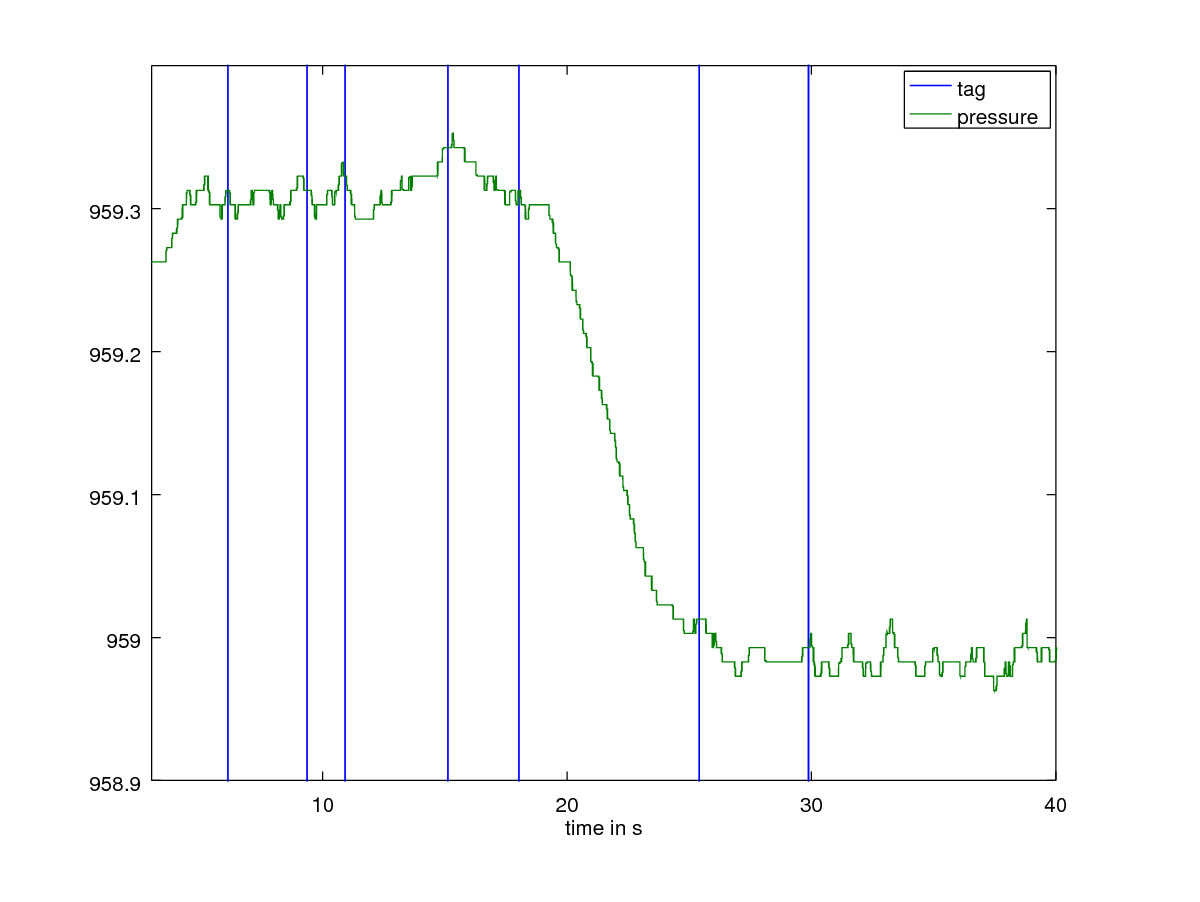
\includegraphics[width=.45\textwidth]{elevupyyikk2_p} &
		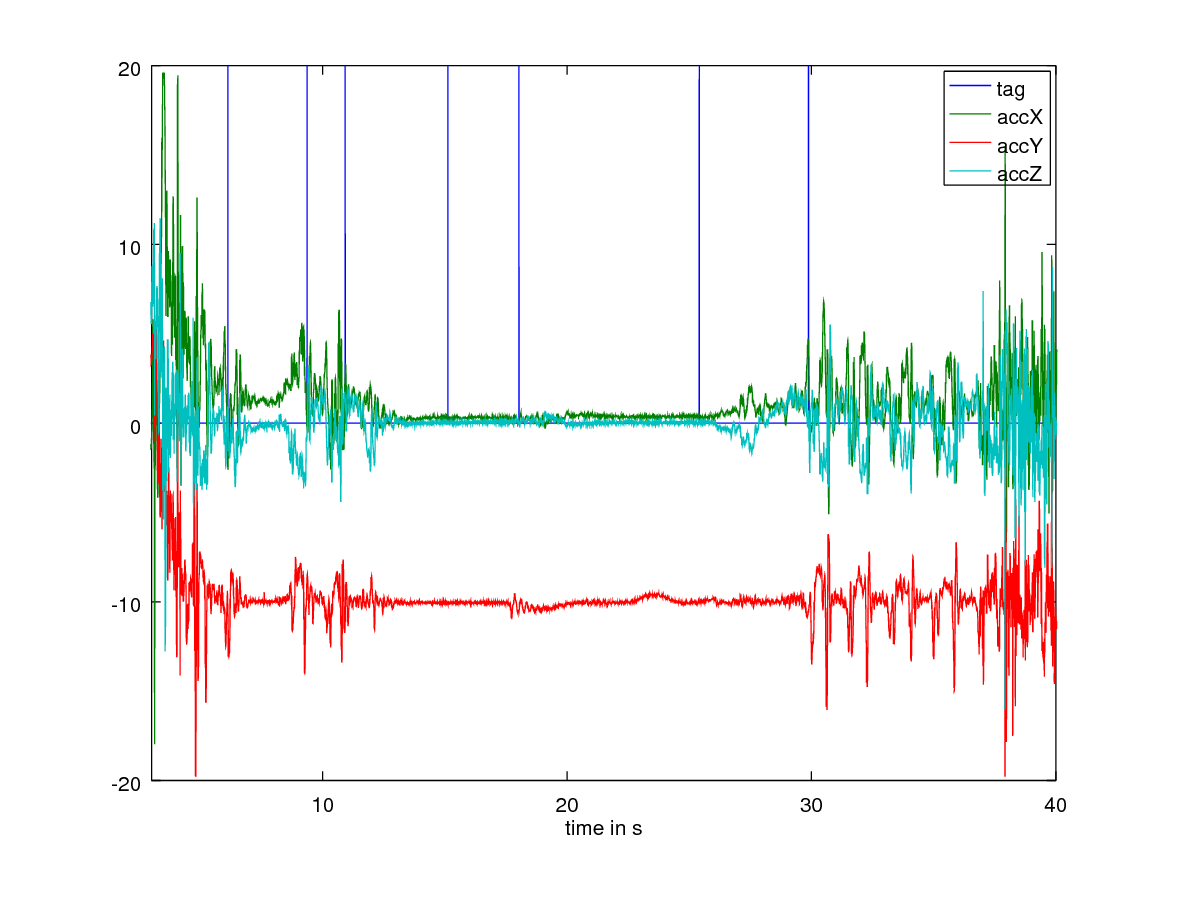
\includegraphics[width=.45\textwidth]{elevupyyikk2_a} 
		\\
		(a) & (b)
		\\[4pt]	%vertical extra spacing (4 points)
		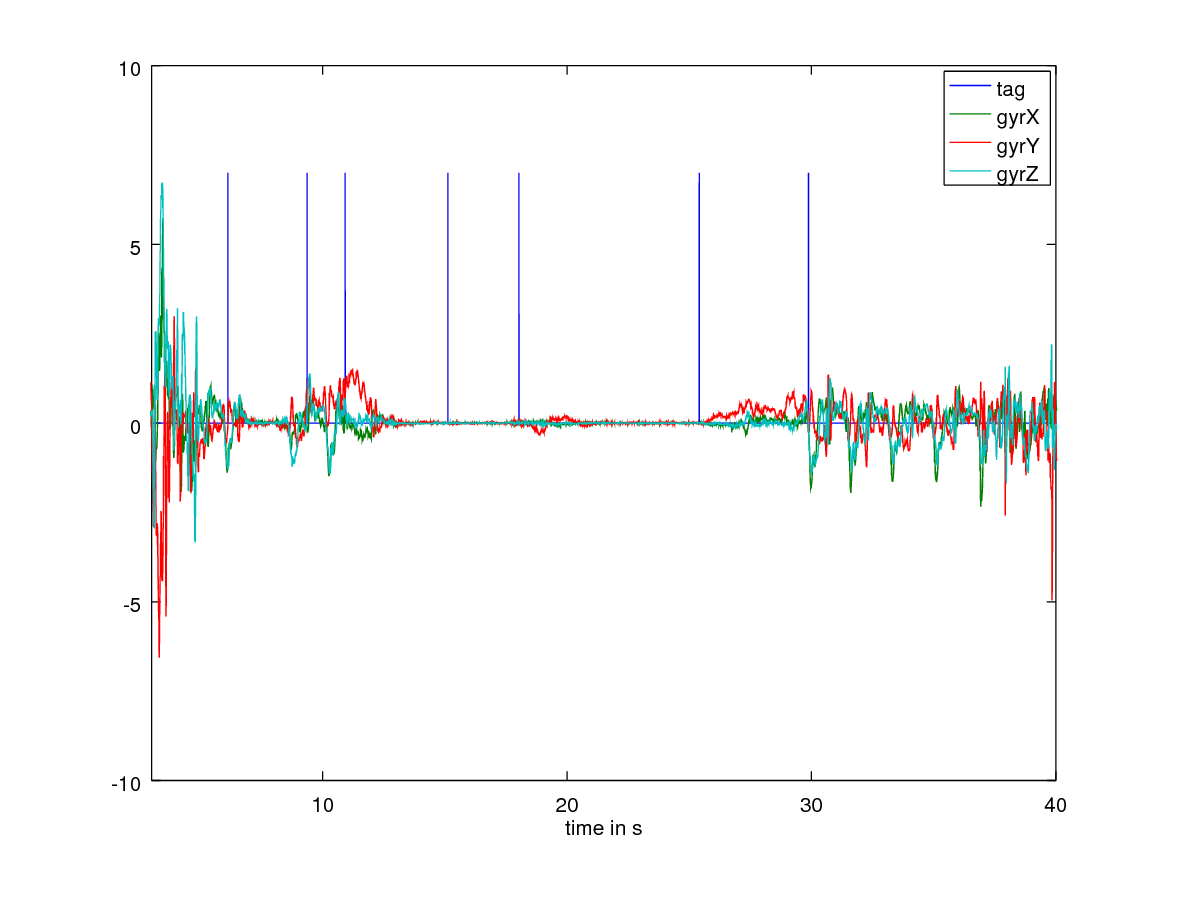
\includegraphics[width=.45\textwidth]{elevupyyikk2_g} &
		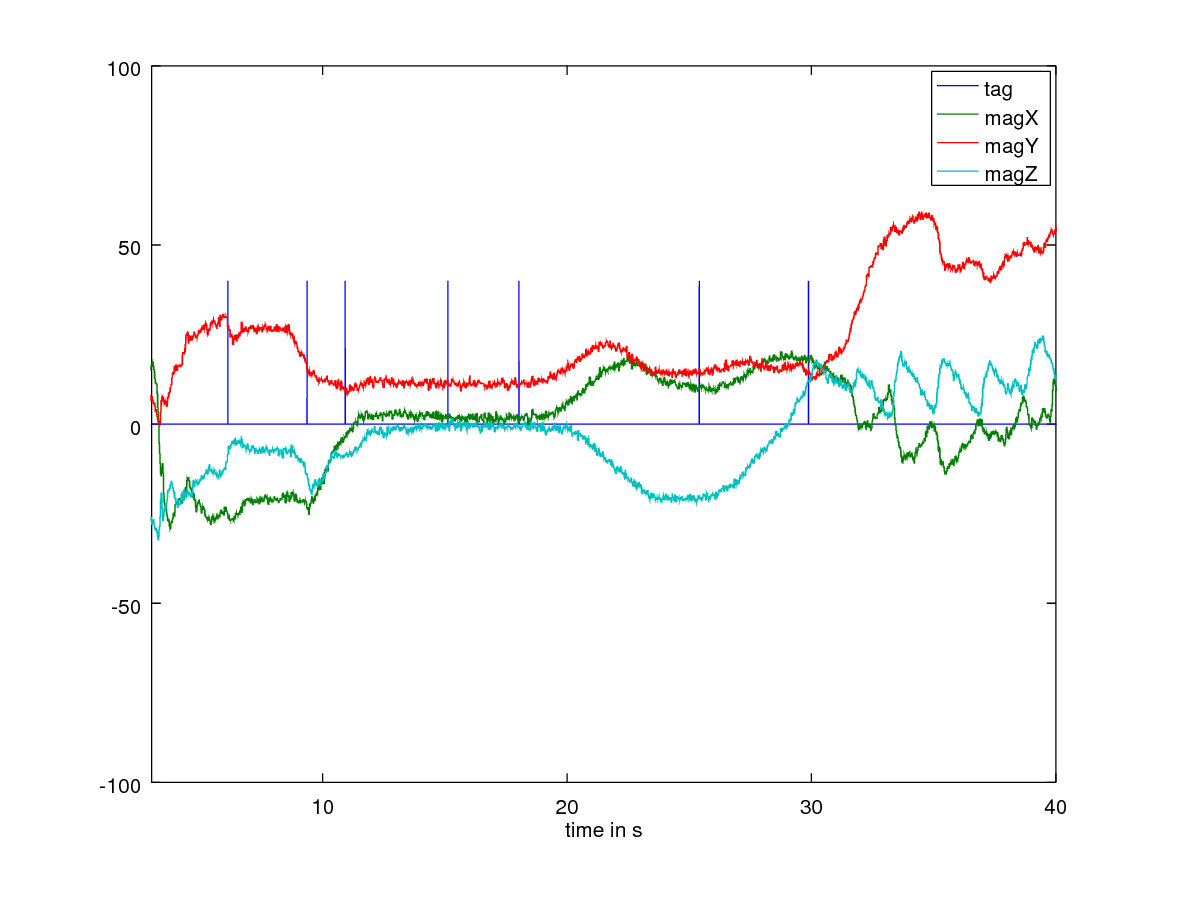
\includegraphics[width=.45\textwidth]{elevupyyikk2_m} 
		\\
		(c) & (d)

	\end{tabular}
	%
	\caption{Test case 10}
	\label{fig:Test_case_elevator_10}
\end{figure}